% Graph Hierarchical Borrowing: companion methods paper to the survey "Collectively Big, Locally Small".
% Submission format: ACM Transactions on Computing for Healthcare (review mode). For a preprint without ACM
% metadata, swap the two \documentclass lines. Figures, generated numbers, the bibliography and the simulation
% code are shared with the survey in../Collectively_Big_Locally_Small.
\documentclass[acmsmall,screen,review]{acmart}
% \documentclass[acmsmall,screen,nonacm]{acmart}
\acmJournal{HEALTH}
\setcopyright{none}

\citestyle{acmauthoryear}
% Generated by simulations/make_numbers.py. Do not edit.
\newcommand{\SimOneChecks}{101}
\newcommand{\SimOneWithin}{98\%}
\newcommand{\SimOneMaxRel}{1.6\%}
\newcommand{\SimOneReps}{40{,}000}
\newcommand{\SimTwoWorstGHB}{1.02}
\newcommand{\SimTwoWorstPool}{382}
\newcommand{\SimTwoMeanPool}{134}
\newcommand{\SimTwoMinGHB}{0.12}
\newcommand{\SimTwoMinOracle}{0.07}
\newcommand{\SimThreeB}{46}
\newcommand{\SimThreeSmall}{2.28}
\newcommand{\SimThreeLarge}{1.08}
\newcommand{\SimThreeMin}{1.05}
\newcommand{\SimThreePoolSmall}{1.44}
\newcommand{\SimThreePoolLarge}{0.15}
\newcommand{\SimThreeKThreeOracle}{0.78}
\newcommand{\SimThreeKThreeDL}{0.91}
\newcommand{\SimThreeKThreeBayes}{0.93}
\newcommand{\SimThreeKFortyEightDL}{0.68}
\newcommand{\SimThreeKFortyEightOracle}{0.66}
\newcommand{\SimFourRingLam}{0.977}
\newcommand{\SimFourRingPred}{203}
\newcommand{\SimFourRingTwo}{35}
\newcommand{\SimFourRegionalLam}{0.964}
\newcommand{\SimFourRegionalPred}{127}
\newcommand{\SimFourRegionalTwo}{22}
\newcommand{\SimFourRandomLam}{0.937}
\newcommand{\SimFourRandomPred}{73}
\newcommand{\SimFourRandomTwo}{11}
\newcommand{\SimFourTwohopLam}{0.933}
\newcommand{\SimFourTwohopPred}{69}
\newcommand{\SimFourTwohopTwo}{14}
\newcommand{\SimFiveMixedGOneEpsTenth}{19.3}
\newcommand{\SimFiveMixedGOneEpsOne}{43.7}
\newcommand{\SimFiveMixedGEightEpsTenth}{21.0}
\newcommand{\SimFiveMixedGEightEpsOne}{45.0}
\newcommand{\SimFiveSmallGOneEpsTenth}{1.0}
\newcommand{\SimFiveSmallGOneEpsOne}{30.6}
\newcommand{\SimFiveSmallGEightEpsTenth}{6.9}
\newcommand{\SimFiveSmallGEightEpsOne}{41.4}
\newcommand{\SimSixGHBLow}{0.31}
\newcommand{\SimSixGMRFLow}{0.40}
\newcommand{\SimSixGHBHigh}{0.94}
\newcommand{\SimSixGMRFHigh}{0.40}
\newcommand{\SimSixBeta}{46}
\newcommand{\SimSevenLocal}{0.0266}
\newcommand{\SimSevenGHB}{0.0182}
\newcommand{\SimSevenGlobal}{0.0173}
\newcommand{\SimSevenReduction}{31\%}
\newcommand{\SimSevenGHBNoDP}{0.0110}
\newcommand{\SimSevenGHBTenth}{0.0285}
\newcommand{\SimSevenLocalTenth}{0.0273}
\newcommand{\SimSevenWorstRatio}{0.94}
\newcommand{\SimSevenGlobalWorstRatio}{2.48}


\usepackage{tabularx}
\usepackage{enumitem}
\usepackage{makecell}
\setlist[enumerate]{itemsep=2pt}
\usepackage{pifont}
\usepackage[ruled,vlined,linesnumbered]{algorithm2e}
\SetAlFnt{\small}
\usepackage{tikz}
\usetikzlibrary{arrows.meta,positioning}
\graphicspath{{../Collectively_Big_Locally_Small/}}

% Colours of the TikZ figures (shared with the survey)
\definecolor{edgec}{rgb}{0.3851,0.41255,0.44}
\definecolor{slate100}{rgb}{0.9451,0.96078,0.97647}
\definecolor{red100}{rgb}{0.99608,0.88628,0.88628}
\definecolor{teal100}{rgb}{0.8,0.98431,0.9451}
\definecolor{blue100}{rgb}{0.85883,0.91765,0.99608}
\definecolor{amber100}{rgb}{0.99608,0.95294,0.7804}
\definecolor{violet100}{rgb}{0.92941,0.91374,0.99608}
\definecolor{famO}{rgb}{0.7255,0.1098,0.1098}
\definecolor{famE}{rgb}{0.14511,0.38824,0.92157}
\definecolor{famT}{rgb}{0.85098,0.46667,0.02353}
\definecolor{famC}{rgb}{0.05882,0.46275,0.43137}
\definecolor{violetc}{rgb}{0.48627,0.22745,0.92941}
\definecolor{grayc}{rgb}{0.60393,0.64706,0.69412}

\newcommand{\eff}{\mathrm{eff}}
\newcommand{\yes}{\textcolor{famC}{\ding{51}}}
\newcommand{\no}{\textcolor{famO}{\ding{55}}}
\newcommand{\partly}{\textcolor{famT}{$\boldsymbol{\circ}$}}

\AtEndPreamble{%
 \theoremstyle{acmdefinition}
 \newtheorem{remark}[theorem]{Remark}}

\begin{document}

\title{Borrowing Strength Without Borrowing Data}
\subtitle{Private, Serverless and Tuning-Free Collaboration with Graph Hierarchical Borrowing}

\author{Sancho Amaral Sim\~{o}es}
\authornote{Corresponding author.}
\email{sanchosimoes@student.dei.uc.pt}
\affiliation{%
 \institution{CISUC, DEI, FCTUC, University of Coimbra}
 \city{Coimbra}
 \country{Portugal}}

\author{Jo\~{a}o P. Vilela}
\email{jvilela@fc.up.pt}
\affiliation{%
 \institution{CISUC, DEI, FCTUC, University of Coimbra}
 \city{Coimbra}
 \country{Portugal}}
\affiliation{%
 \institution{CRACS/INESC TEC, DCS, FCUP, University of Porto}
 \city{Porto}
 \country{Portugal}}

\author{Pedro Henriques Abreu}
\email{pha@dei.uc.pt}
\affiliation{%
 \institution{CISUC, DEI, FCTUC, University of Coimbra}
 \city{Coimbra}
 \country{Portugal}}

\begin{abstract}
Most clinical prediction tasks are small at the hospital that needs the model, while the data that would make them large sit in other hospitals that cannot share patient records and have no centre they all trust. We propose Graph Hierarchical Borrowing (GHB): each hospital shrinks its own model head toward a leave-one-out estimate of the network, by an amount that its own data decide. In a Gaussian random-effects model, every hospital gains almost the same number of ``virtual patients'', $\sigma^2/(\tau^2+M)$, so the smallest hospitals gain the most; differential privacy enters only through the error $M$ of the network estimate; and computing that estimate by gossip over the agreement graph costs no privacy. For realistic heads, the network releases two privatized sums, of every patient's score and information, by secure summation without a server. Each hospital turns them locally into a leave-one-out prior with the privacy noise propagated, and integrates the unknown heterogeneity out against its own evidence. Nothing is tuned. A lighter variant, GHB-lite, in which each hospital releases on its own, is the more accurate where its assumptions hold exactly, in simulation, and falls back to local estimation on small real networks. On five cancer networks from The Cancer Genome Atlas held out from its development, GHB reduced held-out log-loss to \SimTCOneGHB{} of local estimation at $\epsilon=1$ and \SimTCTenGHB{} at $\epsilon=10$, below six federated and personalized methods tuned on twelve other networks (\SimTCOneFT{} and \SimTCTenDitto), and below or level with them tuned on the test patients themselves (\SimTCOneFTOrc{} and \SimTCTenDittoOrc). Stress tests locate the lead: it survives fewer hospitals and larger heads, but comes from fitting related networks together; fitted alone, a network gives GHB only the accuracy of a well-regularized hospital at $\epsilon=1$ and less than Ditto at $\epsilon=10$. The lead is not universal: on the FLamby benchmark GHB is the most accurate method in some settings and not in others, and on Camelyon17 histopathology, with a frozen public encoder, it leads a hospital alone (balanced accuracy \SimCamTenGHB{} against \SimCamLocal) and the tuned literature (\SimCamTenBestReal) only by small margins. Formal tests establish GHB's gain over a hospital alone across all sixteen real data sets, but not, with five held-out networks, its lead over the tuned literature.
\end{abstract}

\begin{CCSXML}
<ccs2012>
  <concept>
    <concept_id>10010147.10010257</concept_id>
    <concept_desc>Computing methodologies~Machine learning</concept_desc>
    <concept_significance>500</concept_significance>
    </concept>
  <concept>
    <concept_id>10010405.10010444.10010449</concept_id>
    <concept_desc>Applied computing~Health informatics</concept_desc>
    <concept_significance>500</concept_significance>
    </concept>
  <concept>
    <concept_id>10002978.10003029.10011150</concept_id>
    <concept_desc>Security and privacy~Privacy protections</concept_desc>
    <concept_significance>500</concept_significance>
    </concept>
 </ccs2012>
\end{CCSXML}

\ccsdesc[500]{Computing methodologies~Machine learning}
\ccsdesc[500]{Applied computing~Health informatics}
\ccsdesc[500]{Security and privacy~Privacy protections}

\keywords{small data, multi-site learning, decentralized learning, gossip, differential privacy, empirical Bayes, hierarchical models, personalization, data silos, healthcare}

\maketitle
\renewcommand{\shortauthors}{Sim\~{o}es et al.}


%% ===================================================================
\section{Introduction}\label{sec:intro}

Most clinical learning problems are small where the model is needed. More than six thousand rare diseases affect 3.5\% to 5.9\% of the population, mostly in cohorts of tens or hundreds of patients \cite{nguengangwakap2020estimating,schaefer2020use}; prediction models in common conditions are routinely built on a few dozen outcome events \cite{peduzzi1996simulation,riley2019minimumsample}; almost none of the hundreds of COVID-19 models built from small local samples was fit for clinical use \cite{roberts2021common,wynants2020prediction}; and deployed systems degrade at the point of use \cite{wong2021external,zech2018variable}. Healthcare is \emph{collectively big and locally small} \cite{simoes2026collectively}: the data that would close the gap exist, but in other hospitals.

Mesothelioma shows the problem in miniature. In The Cancer Genome Atlas \cite{weinstein2013cancer}, the \SimMesoHosp{} institutions that contributed eligible patients hold \SimMesoMin{} to \SimMesoMax{} patients each, \SimMesoPatients{} in all. None can fit even an eight-coefficient model of two-year mortality on its own patients with any confidence; together they hold several times more information, and the same institutions treat other cancers, so what one disease teaches about age or stage can inform another. The question is how such hospitals can learn from each other's patients without seeing them.

Those hospitals cannot simply pool. Training on another hospital's records is secondary use, which needs its own legal basis and often excludes exporting patient-level data; the agreements that allow it are bilateral, slow and partial, so they form a sparse network, and often no institution is trusted or funded to be its centre \cite{cohen2018hipaa,ehds2025,gdpr2016,price2019privacy}. The smallest hospitals, which need collaboration most, are also the easiest to re-identify \cite{rocher2019estimating}. Existing methods each give up something this setting cannot spare. Federated learning needs a trusted server and fits one model \cite{mcmahan2017communication}; personalized variants fit one model per site but keep the server and must tune how much each site borrows \cite{li2021ditto}; decentralized learning removes the server but, in healthcare, lacks formal privacy or shares full models \cite{kalra2023decentralized,warnatherresthal2021swarm}; and private versions of all of them spend the budget over many rounds, with noise largest at the smallest sites \cite{bagdasaryan2019differential,mcmahan2018learning}. Meta-analysis is exact and auditable, but estimates a single population model \cite{dersimonian1986meta}.

\emph{Graph Hierarchical Borrowing} (GHB) starts from an old idea, shrinking each unit's estimate toward what the others suggest by an amount set by how much the units differ \cite{efron1973steins,stein1956inadmissibility}, and asks what it costs when the others' suggestion must be private and computed without a server. The network releases two privatized sums over all of its patients, by secure summation and gossip over the agreement graph. Each hospital turns them, locally and at no further privacy cost, into a leave-one-out prior for its own head and combines it with its own noise-free data, with a weight that its own evidence decides. Privacy noise therefore touches only what a hospital borrows, and is calibrated to the whole network rather than to the smallest hospital. This is how small data can help small data: what a hospital borrows is set by the network's total, not by any one partner, so twenty hospitals of thirty patients give each of them access to six hundred, discounted by how much they differ. The smallest hospitals gain the most, in theory (Section~\ref{sec:borrowing}) and on real networks (Section~\ref{sec:real-tcga}).

\paragraph{Contributions} (1) A formal setting: five requirements for a sparse, serverless network of small hospitals, which no existing approach meets together (Sections~\ref{sec:related} and~\ref{sec:problem}). (2) Closed-form theory: every hospital gains almost the same number $B=\sigma^2/(\tau^2+M)$ of virtual patients, privacy enters only through $M$, and gossip is free post-processing with a rate set by the spectral gap (Section~\ref{sec:model}). (3) A tuning-free method for likelihood-based heads, GHB, with a privacy guarantee for the whole protocol, and a lighter variant, GHB-lite, that needs no secure summation (Section~\ref{sec:heads}). (4) An evaluation in eighteen simulations against baselines tuned with access to the true loss (Section~\ref{sec:experiments}), and on real hospital networks: seven small networks, five held-out cancer networks, the FLamby benchmark and an image task, against six federated and personalized methods tuned as a consortium could and as no consortium can (Section~\ref{sec:real}), with formal tests of every claim under a plan fixed before they were computed. All code and every number are released.

The paper follows one thread. Section~\ref{sec:related} shows what each line of work leaves open, Section~\ref{sec:problem} turns that into requirements, Section~\ref{sec:model} solves the core problem exactly, and Section~\ref{sec:heads} carries the solution to real model heads. Section~\ref{sec:experiments} tests it where the truth is known, Section~\ref{sec:real} where it is not, and Section~\ref{sec:discussion} says when to use it.

%% ===================================================================
\section{Background and Related Work}\label{sec:related}

\subsection{Small data and siloed smallness}\label{sec:smallness}

A dataset is small for a task when the information it carries falls short of what the task needs. The companion survey \cite{simoes2026collectively} measures that information by the \emph{effective sample size}, to first order
\begin{equation}\label{eq:neff}
n^{\eff}=n\cdot\frac{1}{\mathrm{DEFF}}\cdot\rho_L\cdot(1-2\eta)^2\cdot\rho_S,
\end{equation}
with the design effect DEFF of repeated records \cite{kish1965survey}, the labeled fraction $\rho_L$, the label noise $\eta$ \cite{angluin1988learning} and the shift $\rho_S$ to the population of use, and compares it with the sample complexity of the task \cite{riley2019minimumsample}. A task is \emph{siloed-small} when every custodian's data are small for it but their union, after accounting for heterogeneity, is not. The obstacle is then access, not data, and the gain from collaboration is naturally counted in effective patients, which is how Section~\ref{sec:model} counts it.

\subsection{Distributed statistics and empirical Bayes}\label{sec:distributed}

Biostatistics fits models across sites without moving records. Random-effects meta-analysis combines site estimates and estimates their heterogeneity $\tau^2$ \cite{dersimonian1986meta}; distributed regression exchanges sufficient statistics or gradients \cite{duan2020learning,gaye2014datashield,jordan2019communication,wu2012grid}; and infrastructures such as OHDSI \cite{hripcsak2015observational} and the Personal Health Train \cite{beyan2020distributed,deist2020distributed} send analyses to the data. These are exact and auditable, but estimate one population model, offer disclosure controls rather than formal privacy, and mostly assume a coordinator. Empirical Bayes adds the missing step: shrinking each site's estimate toward the population dominates separate estimation \cite{efron1973steins,gelman2013bayesian,stein1956inadmissibility}. This is GHB's statistical core. What is open is its cost when the population estimate must be private and serverless, and its robustness when $\tau^2$ must be estimated from noisy releases.

\subsection{Federated and personalized learning}\label{sec:federated}

Federated averaging trains one model by alternating local steps with averaging at a server \cite{mcmahan2017communication}, and has reached near-pooled quality in medical imaging and clinical prediction \cite{dayan2021federated,pati2022federated,rieke2020future,sheller2020federated}; FLamby provides cross-silo healthcare benchmarks \cite{ogierduterrail2022flamby}. Under heterogeneity the averaged model can be worse than local ones \cite{hsieh2020non,zhao2018federated}, and corrections \cite{karimireddy2020scaffold,li2020federated,li2021fedbn,mohri2019agnostic} still produce one model. Personalized methods learn one model per site through multi-task learning, meta-learning, proximal regularization, shared representations or clusters \cite{collins2021exploiting,deng2020adaptive,fallah2020personalized,ghosh2020efficient,li2021ditto,smith2017federated,tdinh2020personalized}; the theory of shared representations explains why a common representation reduces each site to a small head \cite{du2021few,maurer2016benefit,tripuraneni2020theory}, the split GHB adopts. They keep the server, and how strongly each site relies on the others is a hyperparameter tuned on validation data that small sites lack. Fairness here has two meanings. Fairness across sites, that no site is badly served \cite{li2021ditto,mohri2019agnostic}, is what this paper measures throughout, as each hospital's error relative to its own local estimate. Fairness across patient groups \cite{salazar2023fairfate} needs a protected attribute and a fairness metric; GHB does not target it, and Section~\ref{sec:sim-fairness} measures what borrowing does to it.

\subsection{Decentralized learning}\label{sec:decentralized}

Decentralized SGD and gossip replace the server by neighbour averaging, with rates set by the spectral gap of the graph \cite{boyd2006randomized,koloskova2020unified,lian2017can,nedic2009distributed,xiao2004fast}; personalized versions use a similarity graph \cite{bellet2018personalized,vanhaesebrouck2017decentralized}, and decentralization amplifies privacy \cite{cyffers2022privacy}. Healthcare examples, Swarm Learning \cite{warnatherresthal2021swarm}, ProxyFL \cite{kalra2023decentralized} and peer-to-peer segmentation \cite{roy2019braintorrent,tedeschini2022decentralized}, either lack formal privacy by default or share full models, and none models heterogeneity explicitly.

\subsection{Privacy in multi-site learning}\label{sec:dp}

Gradients and models leak training data \cite{geiping2020inverting,hatamizadeh2023do,shokri2017membership,zhu2019deep}. Differential privacy bounds what any output reveals about one patient \cite{dwork2006calibrating,dwork2014algorithmic}, extends to deep and federated learning \cite{abadi2016deep,mcmahan2018learning,mironov2017renyi}, and composes tightly under zero-concentrated accounting \cite{bun2016concentrated}. Its noise is calibrated to sensitivity, which grows as sample size shrinks, so it costs most for small datasets and large models \cite{bagdasaryan2019differential,tramer2021differentially}. Secure aggregation reveals only sums \cite{bonawitz2017practical}. For small hospitals, a method that releases often, releases large objects or calibrates noise to each site cancels the benefit of collaboration.

\subsection{What is missing}\label{sec:gap}

Each line supplies a piece: exact population estimation, the optimal combination with each site, the representation and head split, serverless computation and a formal guarantee. Missing is their combination: a method that spends privacy once, at the network level, personalizes without tuning, runs over whatever agreements exist, and states its benefit to each hospital in advance.

%% ===================================================================
\section{Problem Setting}\label{sec:problem}

There are $K$ hospitals, the vertices of a connected undirected graph $\mathcal{G}=(V,E)$ whose edges are agreements to exchange privatized summaries; $\mathcal{G}$ is sparse ($|E|=O(K)$) and no vertex is trusted by all. Hospital $k$ holds $n_k$ labeled records from its population $P_k$ and wants a model for that population. We require:
\begin{enumerate}[label=(R\arabic*),leftmargin=*,itemsep=1pt]
\item no patient-level record leaves its hospital;
\item every released quantity satisfies $(\epsilon,\delta)$-differential privacy with respect to the patients of the releasing hospital;
\item no central server: computation uses only messages along edges of $\mathcal{G}$;
\item the smallest hospitals benefit at least as much as the largest, in relative terms;
\item heterogeneity across hospitals is modeled rather than assumed away.
\end{enumerate}
(R4) and (R5) exclude a single global model, which serves the typical site and charges its privacy cost to the smallest. Existing data-exchange agreements do not remove the problem: they mostly serve primary care, and agreements for secondary use form exactly the sparse graph assumed here \cite{ehds2025,gdpr2016}. GHB runs over them, and infrastructures such as OHDSI, DataSHIELD and the Personal Health Train \cite{beyan2020distributed,gaye2014datashield,hripcsak2015observational} can carry its messages. Where a trusted environment for pooling exists, (R3) is moot and the borrowing of Section~\ref{sec:borrowing} can run inside it without noise.

\paragraph{Threat model} GHB protects patients against honest-but-curious hospitals and any observer of the messages. Its joint releases use secure summation, which assumes that hospitals do not collude to remove their noise shares (Proposition~\ref{prop:ghbprivacy} states what collusion costs); GHB-lite needs no such assumption. Hospitals follow the protocol; Section~\ref{sec:sim-attacks} tests what lies do. Site sizes are public.

\paragraph{Why not anonymize?} Anonymization, removing identifiers or generalizing records until each matches $k$ others \cite{sweeney2002k}, is the usual answer to sharing health data, and GHB deliberately does not rely on it. Patient records never leave the hospital, so there is nothing to anonymize; what leaves are two noisy sums over the whole network. And anonymization fails on the data it would apply to: rich health records are re-identified from a handful of attributes \cite{rocher2019estimating}, and its protection, unlike that of differential privacy, does not survive the combination of several releases or the attacker's background knowledge \cite{dwork2014algorithmic,ganta2008composition}. Differential privacy instead bounds what any release can reveal about any one patient, whatever else is known, and Section~\ref{sec:real-reid} measures that bound and the risk that remains on real data.

\paragraph{How existing approaches fare} Table~\ref{tab:approaches} compares design properties, not performance. Pooling violates (R1); federated averaging violates (R3) and, under heterogeneity, (R4) and (R5); personalized learning keeps the server; Swarm Learning lacks formal privacy and ProxyFL shares full models; synthetic data trades utility for privacy \cite{jordon2019pate,stadler2022synthetic}; meta-analysis ignores representations and graph structure. GHB meets all five by construction, under the assumptions of Propositions~\ref{prop:borrowing}, \ref{prop:gossip} and~\ref{prop:ghbprivacy}; whether it also performs is the subject of Sections~\ref{sec:experiments} and~\ref{sec:real}.

\begin{table}[t]
\caption{Approaches for sparse, siloed hospital networks against requirements (R1) to (R5), as design properties of each method in its standard form. \yes{} satisfied; \partly{} partially or optionally; \no{} not satisfied. Entries for GHB hold by construction under the assumptions of Sections~\ref{sec:model} and~\ref{sec:algorithm}; (R2) and (R3) assume secure summation by hospitals that do not collude (Proposition~\ref{prop:ghbprivacy}).}
\label{tab:approaches}
\small
\begin{tabularx}{\linewidth}{@{}>{\raggedright\arraybackslash}Xccccc@{}}
\toprule
Approach & \shortstack{(R1)\\local data} & \shortstack{(R2)\\formal DP} & \shortstack{(R3)\\no server} & \shortstack{(R4)\\small sites gain} & \shortstack{(R5)\\heterogeneity}\\
\midrule
Centralized pooling & \no & \no & \no & \partly & \partly\\
Federated averaging \cite{mcmahan2017communication} & \yes & \partly & \no & \no & \no\\
Personalized FL \cite{collins2021exploiting,li2021ditto} & \yes & \partly & \no & \yes & \yes\\
Swarm Learning \cite{warnatherresthal2021swarm} & \yes & \no & \yes & \partly & \no\\
ProxyFL \cite{kalra2023decentralized} & \yes & \yes & \yes & \partly & \partly\\
Synthetic data sharing \cite{jordon2019pate} & \yes & \partly & \yes & \partly & \no\\
Distributed meta-analysis \cite{dersimonian1986meta,duan2020learning} & \yes & \partly & \partly & \yes & \yes\\
\textbf{GHB (this paper)} & \yes & \yes & \yes & \yes & \yes\\
\bottomrule
\end{tabularx}
\end{table}

%% ===================================================================
\section{Hierarchical Borrowing in a Model That Can Be Solved Exactly}\label{sec:model}

We first solve the core problem in the simplest model that keeps its structure: one parameter per hospital, Gaussian random effects, and a population estimate that must be private and serverless. This gives closed forms for what each hospital gains, what privacy costs and what the absence of a server costs.

\subsection{Borrowing with an imperfect population estimate}\label{sec:borrowing}

How much should a hospital trust what the others suggest, when their suggestion is itself imperfect? Each hospital has a parameter $\theta_k\in\mathbb{R}$ (one coordinate of a head) and an asymptotically normal local estimate:
\begin{equation}\label{eq:model}
\theta_k=\mu+u_k,\quad u_k\sim\mathcal{N}(0,\tau^2);\qquad \hat{\theta}_k=\theta_k+e_k,\quad e_k\sim\mathcal{N}(0,v_k),\quad v_k=\sigma^2/n_k,
\end{equation}
all independent, with heterogeneity $\tau^2$ \cite{dersimonian1986meta} and $\sigma^2$ the inverse Fisher information per patient. Unlike classical empirical Bayes \cite{efron1973steins,gelman2013bayesian}, hospital $k$ only has an estimate $\tilde{\mu}$ of $\mu$, with error.

\begin{figure}[t]
\centering
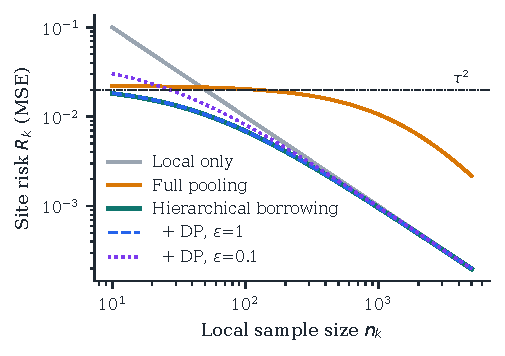
\includegraphics[width=0.49\linewidth]{figures/fig_risk}\hfill
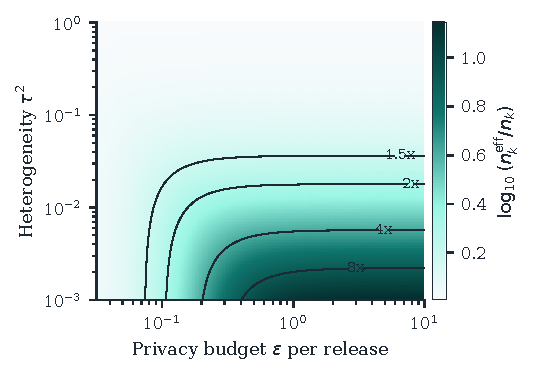
\includegraphics[width=0.49\linewidth]{figures/fig_ess_gain}
\caption{Left: risk of hospital $k$ as a function of its size $n_k$, with $K=12$, other hospitals of 200 patients, $\sigma^2=1$, $\tau^2=0.02$ and $\delta=10^{-5}$. Full pooling is excellent for small sites until it hits the heterogeneity floor $\tau^2$, and then harms large ones; hierarchical borrowing (Proposition~\ref{prop:borrowing}), with $\tau^2$ and $M$ known, is never worse than either in expected risk. Privacy at $\epsilon=1$ is almost free; at $\epsilon=0.1$ it reduces but does not remove the gain. Right: relative gain in effective sample size $n^{\eff}_k/n_k$ for a hospital with $n_k=50$, as a function of heterogeneity and privacy budget, from Equations~\eqref{eq:borrowed} and~\eqref{eq:M}.}
\label{fig:risk}
\end{figure}

\begin{proposition}[Borrowing with an imperfect prior]\label{prop:borrowing}
Let $\tilde{\mu}$ be any estimate of $\mu$ that is independent of $(u_k,e_k)$ and has mean squared error $M=\mathbb{E}(\tilde{\mu}-\mu)^2$. Among estimators $\tilde{\theta}_k=\alpha\hat{\theta}_k+(1-\alpha)\tilde{\mu}$, the risk $R_k(\alpha)=\mathbb{E}(\tilde{\theta}_k-\theta_k)^2$ is minimized at
\[
\alpha_k^{\star}=\frac{\tau^2+M}{\tau^2+M+v_k},\qquad R_k^{\star}=\frac{v_k\,(\tau^2+M)}{v_k+\tau^2+M}\;\le\;\min\{v_k,\;\tau^2+M\}.
\]
Equivalently, the effective sample size of hospital $k$ becomes
\begin{equation}\label{eq:borrowed}
n_k^{\eff}=\frac{\sigma^2}{R_k^{\star}}=n_k+\underbrace{\frac{\sigma^2}{\tau^2+M}}_{\text{borrowed patients }B}.
\end{equation}
\end{proposition}
\begin{proof}
$\tilde{\theta}_k-\theta_k=\alpha e_k+(1-\alpha)(\tilde{\mu}-\mu)-(1-\alpha)u_k$. The three terms are mutually independent, and the first and last have zero mean, so the cross terms vanish; the middle term has second moment $M$. Hence $R_k(\alpha)=\alpha^2 v_k+(1-\alpha)^2(\tau^2+M)$. This is a convex quadratic in $\alpha$, minimized at $\alpha_k^{\star}$; substituting gives $R_k^{\star}$. The bound follows because $R_k^{\star}$ is half the harmonic mean of $v_k$ and $\tau^2+M$. Finally $\sigma^2/R_k^{\star}=\sigma^2/v_k+\sigma^2/(\tau^2+M)=n_k+B$.
\end{proof}

The proof uses only moments and independence, so normality is not needed. $R_k$ averages over the site effect: a hospital far from the others ($|u_k|\gg\tau$) can lose by borrowing, which is why $\tau^2$ must be learned from the data (Section~\ref{sec:tau}). Equation~\eqref{eq:borrowed} is the central quantity of the method. Every hospital gains almost the same number $B$ of \emph{virtual patients}, whatever its size: a hospital of 30 patients may triple its effective sample, one of 3,000 barely notices, so (R4) holds by construction. These patients come from the network as a whole: $M$ shrinks as the other hospitals' patients add up (Equation~\eqref{eq:M}), so many small hospitals together can give each of them what one large partner would, and $\tau^2$, how much they differ, sets the ceiling $B\le\sigma^2/\tau^2$. As $\tau^2\to\infty$, $B\to0$ and each hospital should act alone; as $\tau^2,M\to0$, full pooling is optimal. With $\tau^2$ and $M$ known, borrowing is never worse than either (Figure~\ref{fig:risk}).

\subsection{The cost of privacy}\label{sec:privacy}

Proposition~\ref{prop:borrowing} holds for any $\tilde{\mu}$; privacy (R2) constrains how it is obtained. A hospital's own estimate never leaves it and needs no noise, so privacy affects only $M$.

\begin{proposition}[Privatized population estimate]\label{prop:privatized}
Suppose $\hat{\theta}_j$ is the mean of per-patient contributions clipped to $[-C,C]$, so that replacing one patient changes $\hat{\theta}_j$ by at most $\Delta_j=2C/n_j$, and that clipping introduces no bias. Each hospital $j$ releases $\hat{\theta}_j+\xi_j$ with $\xi_j\sim\mathcal{N}(0,s_j^2)$ and $s_j=\Delta_j\sqrt{2\ln(1.25/\delta)}/\epsilon$, which is $(\epsilon,\delta)$-differentially private for $\epsilon\in(0,1)$ by the Gaussian mechanism \cite{dwork2014algorithmic}. For the leave-one-out average $\tilde{\mu}=\frac{1}{K-1}\sum_{j\neq k}(\hat{\theta}_j+\xi_j)$,
\begin{equation}\label{eq:M}
M=\frac{1}{(K-1)^2}\sum_{j\neq k}\Bigl(\tau^2+\frac{\sigma^2}{n_j}+\frac{8C^2\ln(1.25/\delta)}{n_j^2\,\epsilon^2}\Bigr).
\end{equation}
\end{proposition}

\begin{proof}
The terms $u_j+e_j+\xi_j$ are independent with zero mean and variances $\tau^2+\sigma^2/n_j+s_j^2$, and $s_j^2=4C^2\cdot 2\ln(1.25/\delta)/(n_j^2\epsilon^2)$. Independence from $(u_k,e_k)$ holds because $k$ is excluded.
\end{proof}

Privacy noise is divided by $K-1$ and vanishes as the network grows, while the local estimate stays noise-free. But it scales as $n_j^{-2}$, against $n_j^{-1}$ for sampling error: per-hospital releases are cheap for large hospitals and ruinous for tiny ones. Releasing \emph{sums} removes that cost, because the sensitivity of a sum is set by one patient, not by the smallest hospital; Section~\ref{sec:logit} builds GHB on this. Five conditions delimit the guarantee: (a) neighbouring datasets differ in one patient at one hospital, so a patient held by $m$ hospitals is protected at $(m\epsilon,m\delta)$; (b) site sizes are public; (c) a head in $\mathbb{R}^p$ is released as one vector with $\ell_2$ clipping, not coordinate by coordinate; (d) for a head fitted by maximum likelihood, the natural release is the mean score at a public point, with sensitivity $2L/n_j$ for an $L$-Lipschitz loss ($L=\max\|x\|$ for logistic regression), mapped back to the parameter by public post-processing (Section~\ref{sec:lite}); (e) refits compose, and zero-concentrated accounting \cite{bun2016concentrated} keeps that composition tight.

\subsection{Computation on a sparse graph without a server}\label{sec:gossip}

Without a server, hospitals average by gossip \cite{boyd2006randomized,xiao2004fast}: with a symmetric doubly stochastic $W$ supported on $E$ (for instance Metropolis-Hastings weights $W_{kl}=1/(1+\max(d_k,d_l))$), each round sets $x^{t+1}=Wx^t$, starting from the privatized releases $x_j^0=\hat{\theta}_j+\xi_j$.

\begin{proposition}[Free post-processing and convergence]\label{prop:gossip}
(i) Every message exchanged during gossip is a function of the privatized releases only, so the whole gossip phase satisfies the same $(\epsilon,\delta)$ guarantee as the initial release, with no additional privacy cost. (ii) Let $\lambda=\max\{|\lambda_2(W)|,|\lambda_K(W)|\}$. If $\mathcal{G}$ is connected and $W$ has a positive diagonal, then $\lambda<1$ and
\[
\bigl\|x^t-\bar{x}\mathbf{1}\bigr\|_2\;\le\;\lambda^t\,\bigl\|x^0-\bar{x}\mathbf{1}\bigr\|_2,
\]
so that the estimate held by any hospital after $t$ rounds has root mean squared error at most $\sqrt{M_{\mathrm{all}}}+\lambda^t\sqrt{\mathbb{E}\|x^0-\bar{x}\mathbf{1}\|_2^2}$ as an estimate of $\mu$, where $M_{\mathrm{all}}=K^{-2}\sum_{j}(\tau^2+\sigma^2/n_j+s_j^2)$ is the mean squared error of the full average. (iii) Hospital $k$ obtains its leave-one-out estimate as $\tilde{\mu}_k^t=(Kx_k^t-x_k^0)/(K-1)$. It converges to the leave-one-out average of Proposition~\ref{prop:privatized}, and differs from it by $K(x_k^t-\bar{x})/(K-1)$, whose root mean square is at most $\frac{K}{K-1}\lambda^t\sqrt{\mathbb{E}\|x^0-\bar{x}\mathbf{1}\|_2^2}$.
\end{proposition}

\begin{proof}
(i) is the post-processing property of differential privacy \cite{dwork2014algorithmic}: the gossip iterates are a deterministic function of the released values, and each hospital's subsequent computations on its own data are never released. (ii) Since $W$ is symmetric and doubly stochastic, $\mathbf{1}$ is an eigenvector with eigenvalue 1 and $x^t-\bar{x}\mathbf{1}=W^t(x^0-\bar{x}\mathbf{1})$ lies in the orthogonal complement of $\mathbf{1}$, on which $\|W\|_2=\lambda$. Connectivity and a positive diagonal make $W$ irreducible and aperiodic, so $\lambda<1$ \cite{xiao2004fast}. The error bound follows from the triangle inequality in $L^2$, since each coordinate deviation is bounded by the norm of the whole vector. (iii) Since $\sum_{j\neq k}x_j^0=K\bar{x}-x_k^0$, the leave-one-out average is $(K\bar{x}-x_k^0)/(K-1)$, and subtracting it from $\tilde{\mu}_k^t$ leaves $K(x_k^t-\bar{x})/(K-1)$, which is bounded as in (ii).
\end{proof}

The rounds needed for accuracy $\gamma$ are about $\log(1/\gamma)/(1-\lambda)$, so the spectral gap sets the communication cost, and a hospital should use its estimate only once $\lambda^t$ is small. Which agreements a network signs matters more than how many: a few long-range links triple the gap of a ring or of regional clusters (Figure~\ref{fig:gossip}).

\begin{figure}[t]
\centering
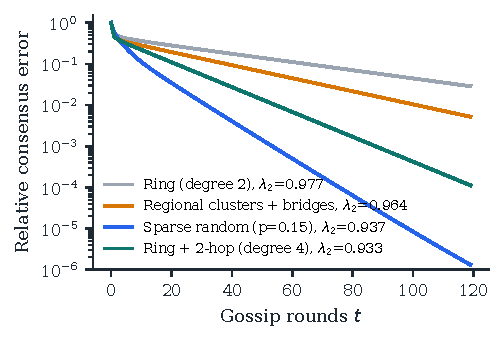
\includegraphics[width=0.6\linewidth]{figures/fig_gossip}
\caption{Gossip consensus error for 24 hospitals on four sparse topologies with Metropolis-Hastings weights. Rates follow the second largest eigenvalue modulus $\lambda$ of the gossip matrix (Proposition~\ref{prop:gossip}).}
\label{fig:gossip}
\end{figure}

\subsection{Unknown heterogeneity}\label{sec:tau}

The propositions take $\tau^2$ as known. How a hospital handles not knowing it decides whether borrowing helps or harms it.

\begin{remark}[Estimating $\tau^2$, or integrating it out]\label{rem:tau}
Moment estimators of $\tau^2$ \cite{dersimonian1986meta} use only the public releases and their variances, so they inherit the guarantee. Better, hospital $k$ can integrate $\tau$ out: take $Q$ equally weighted quantiles $\tau_q$ of its posterior under a half-Cauchy prior, and average its estimates under the priors $\mathcal{N}(\tilde{\mu}_k(\tau_q),\tau_q^2+M_k(\tau_q))$, each weighted by the marginal likelihood of its own data (closed form in the Gaussian model, Laplace otherwise). A hospital whose data agree with the network borrows strongly; one whose data conflict puts its weight on wide components and falls back to its own data. This costs no privacy, since the hospital's data are used only inside it.
\end{remark}

With noisy releases the posterior of $\tau$ is wide: a plug-in posterior mean then overstates heterogeneity and switches borrowing off, and a plug-in median or moment estimate can understate it. Averaging over the posterior, weighted by each hospital's evidence, commits to neither, and Simulation 16 finds it among the largest improvements (Section~\ref{sec:sim-components}).

\subsection{Structured heterogeneity}\label{sec:structured}

When similarity has structure, for instance by region, a Gaussian Markov random field prior \cite{rue2005gaussian} on a similarity graph with weights $a_{kl}$ and Laplacian $L$ gives the maximum a posteriori problem
\begin{equation}\label{eq:gmrf}
\min_{\boldsymbol{\theta}}\;\sum_k\frac{(\theta_k-\hat{\theta}_k)^2}{2v_k}+\frac{\beta}{2}\sum_{k<l}a_{kl}(\theta_k-\theta_l)^2+\frac{\gamma}{2}\sum_k(\theta_k-\mu_0)^2,
\end{equation}
solved by the Jacobi iteration $\theta_k\leftarrow(\hat{\theta}_k/v_k+\beta\sum_l a_{kl}\theta_l+\gamma\mu_0)/(1/v_k+\beta d_k+\gamma)$, which uses only neighbour values and converges because the system is strictly diagonally dominant. It generalizes \citet{vanhaesebrouck2017decentralized} with an anchor $\mu_0$ from published knowledge; neighbours exchange values computed from privatized releases, and each hospital applies the last update with its own data locally.

%% ===================================================================
\section{GHB for Model Heads}\label{sec:heads}

The analysis applies to any parametric head, in particular the last layer on top of a fixed representation. This section places borrowing in an architecture, specifies what the network releases and how each hospital uses it, and states the privacy of the whole protocol.

\subsection{Architecture}\label{sec:architecture}

GHB keeps the privatized part of the model small and surrounds it with components that cost no privacy (Figure~\ref{fig:ghb}), each drawing on a different source of the information a small hospital lacks \cite{simoes2026collectively}:
\begin{enumerate}[label=\textbf{L\arabic*},start=0,leftmargin=*,itemsep=1pt]
\item \textbf{Public representation:} a foundation encoder pretrained on public data \cite{moor2023foundation,rasmy2021med,zhou2023foundation}.
\item \textbf{Local adaptation:} low-rank adapters \cite{hu2022lora} trained self-supervised on the hospital's unlabeled data \cite{chen2020simple,he2022masked}.
\item \textbf{Hierarchical head:} a low-dimensional head $\theta_k\in\mathbb{R}^p$ that borrows by Sections~\ref{sec:model} and~\ref{sec:logit}.
\item \textbf{Knowledge anchor:} a prior mean $\mu_0$ from published models, so that a hospital with no neighbours starts somewhere sensible.
\item \textbf{Site calibration:} conformal prediction on local held-out data \cite{angelopoulos2023conformal,lu2023federated,shafer2008tutorial}.
\item \textbf{Targeted procurement:} posterior variances point to the patients most worth labeling next \cite{settles2009active}.
\end{enumerate}
A small private component is a necessity, not a convenience: Gaussian noise grows with $\sqrt{p}$, and private learning is far more accurate on good fixed features than end to end \cite{tramer2021differentially}. Synthetic data is left out of the training path, since a generator fitted to a hospital's data adds no information about its target \cite{simoes2026collectively,stadler2022synthetic}.

\begin{figure}[t]
\centering
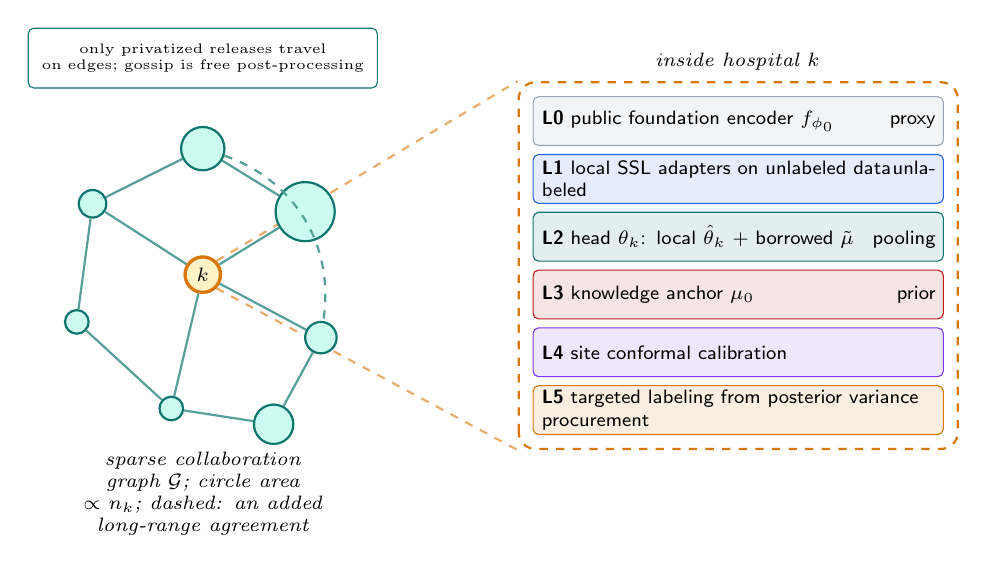
\begin{tikzpicture}[x=1bp,y=1bp,
 hosp/.style={fill=teal100,draw=famC,line width=0.8pt},
 link/.style={draw=famC!70,line width=0.8pt},
 layer/.style={fill=#1!12,draw=#1,line width=0.4pt,rounded corners=2pt},
 ltxt/.style={anchor=west,font=\scriptsize\sffamily,inner sep=0pt,text width=142.26pt}]
% inside-hospital panel
\path[fill=white,draw=famT,line width=0.8pt,dashed,rounded corners=6pt] (-16.674,-62.733) rectangle (141.400,69.244);
\draw[famT!60,line width=0.8pt,dashed] (-125.46,4.93) -- (-17.07,69.64);
\draw[famT!60,line width=0.8pt,dashed] (-125.46,-4.93) -- (-17.07,-63.13);
% hospitals (circle area proportional to n_k)
\path[hosp] (-130.395,45.355) circle (7.795);
\path[hosp] (-170.080,25.510) circle (4.960);
\path[hosp] (-93.540,22.680) circle (10.630);
\path[hosp] (-175.750,-17.010) circle (4.250);
\path[fill=amber100,draw=famT,line width=1.2pt] (-130.395,0) circle (6.375);
\path[hosp] (-87.875,-22.680) circle (5.665);
\path[hosp] (-141.735,-48.190) circle (4.250);
\path[hosp] (-104.885,-53.860) circle (7.085);
\node[inner sep=0pt,font=\scriptsize] at (-130.395,0) {$k$};
% agreements
\draw[link] (-137.72,41.69) -- (-165.29,27.91);
\draw[link] (-123.42,41.06) -- (-102.94,28.46);
\draw[link] (-170.79,20.20) -- (-175.14,-12.40);
\draw[link] (-165.57,22.61) -- (-136.26,3.77);
\draw[link] (-124.45,3.66) -- (-102.94,16.90);
\draw[link] (-124.24,-3.28) -- (-93.23,-19.82);
\draw[link] (-172.32,-20.15) -- (-145.16,-45.05);
\draw[link] (-137.14,-48.90) -- (-112.28,-52.72);
\draw[link] (-101.30,-47.29) -- (-90.78,-28.00);
\draw[link] (-131.99,-6.79) -- (-140.67,-43.66);
\draw[link,dashed] (-122.60,42.82).. controls (-96.997,33.945) and (-82.733,10.089).. (-87.031,-16.669);
\node[align=center,font=\scriptsize\itshape,text width=95pt,anchor=north] at (-130.395,-60.34) {sparse collaboration graph $\mathcal{G}$; circle area $\propto n_k$; dashed: an added long-range agreement};
% layers
\path[layer=grayc] (-11.493,46.489) rectangle (136.219,64.064);
\path[layer=famE] (-11.493,25.680) rectangle (136.219,43.255);
\path[layer=famC] (-11.493,4.870) rectangle (136.219,22.450);
\path[layer=famO] (-11.493,-15.940) rectangle (136.219,1.640);
\path[layer=violetc] (-11.493,-36.740) rectangle (136.219,-19.170);
\path[layer=famT] (-11.493,-57.550) rectangle (136.219,-39.980);
\node[ltxt] at (-8.50,55.276) {\textbf{L0} public foundation encoder $f_{\phi_0}$\hfill proxy};
\node[ltxt] at (-8.50,34.467) {\textbf{L1} local SSL adapters on unlabeled data\hfill unlabeled};
\node[ltxt] at (-8.50,13.660) {\textbf{L2} head $\theta_k$: local $\hat{\theta}_k$ + borrowed $\tilde{\mu}$\hfill pooling};
\node[ltxt] at (-8.50,-7.150) {\textbf{L3} knowledge anchor $\mu_0$\hfill prior};
\node[ltxt] at (-8.50,-27.955) {\textbf{L4} site conformal calibration};
\node[ltxt] at (-8.50,-48.765) {\textbf{L5} targeted labeling from posterior variance\hfill procurement};
\node[anchor=base,font=\scriptsize\itshape,inner sep=0pt] at (62.08,74.82) {inside hospital $k$};
% note
\path[fill=white,draw=famC,line width=0.4pt,rounded corners=2pt] (-193.24,67.20) rectangle (-67.55,88.71);
\node[align=center,font=\tiny,inner sep=0pt,text width=4.3cm] at (-130.395,77.955) {only privatized releases travel\\ on edges; gossip is free post-processing};
\end{tikzpicture}
\caption{Graph Hierarchical Borrowing (GHB). Left: hospitals of very different sizes connected by a sparse set of agreements, without a central server. Right: the model held by each hospital, with the source of information used at each layer. Only the low-dimensional head participates in privatized exchange.}
\label{fig:ghb}
\end{figure}

\subsection{What the network releases}\label{sec:logit}

Section~\ref{sec:privacy} showed that noise calibrated to a sum is set by one patient, not by the smallest hospital. GHB applies this to the whole network: it makes two joint releases, sums over every patient of every hospital, revealed only as totals, and computes everything else from them, from public information and, inside each hospital, from its own data.

\paragraph{Two joint releases} Let $G=\max\|x\|$ bound the features of a likelihood-based head. For logistic regression the per-patient score at the origin is $\psi_i=x_i(y_i-\tfrac12)$ and the information is $\phi_i=x_ix_i^{\top}/4$. The network releases
\[
\tilde{S}=\sum_{k}\sum_{i\in k}\psi_i+\xi,\quad \xi\sim\mathcal{N}(0,s_S^2I_p),\qquad
\tilde{J}=\sum_{k}\sum_{i\in k}\phi_i+E,\quad E_{ab}=E_{ba}\sim\mathcal{N}(0,s_J^2)\ (a\le b).
\]
Replacing one patient moves $\sum\psi_i$ by at most $2G$. Since the $\phi_i$ are positive semidefinite with Frobenius norm at most $G^2/4$, and $\|A-B\|_F^2\le\|A\|_F^2+\|B\|_F^2$ for positive semidefinite $A,B$, it moves the upper triangle of $\sum\phi_i$ by at most $\sqrt2\,G^2/4$. Each release gets half of a zero-concentrated budget $\rho$, so $s_S=2G/\sqrt{\rho}$ and $s_J=\sqrt2\,G^2/(4\sqrt{\rho})$, with $\rho+2\sqrt{\rho\ln(1/\delta)}=\epsilon$ \cite{bun2016concentrated}. When the matrix would be mostly noise, only its diagonal is released, by a public rule fixed in advance: the diagonal when $s_J\sqrt{p}>NG^2/(4p)$. The sums are computed by secure summation \cite{bonawitz2017practical}: neighbours agree on pairwise masks that cancel in the total, every hospital adds its masked contribution and a share $\mathcal{N}(0,s^2/K)$ of the noise, and gossip averages the masked values (Proposition~\ref{prop:gossip}), so no server is needed and no hospital's contribution is revealed.

\paragraph{From the releases to the network} With $A=(\tilde{J}^{+}+I/s_0^2)^{-1}$, where $\tilde{J}^{+}$ is $\tilde{J}$ projected onto the positive semidefinite cone and $s_0=2.5$ is the weakly informative default scale for logistic coefficients \cite{gelman2008weakly}, the network estimate is one Newton step of the pooled model from the origin, $\hat{w}=A\tilde{S}$, with public privacy covariance $V_{\mathrm{dp}}=s_S^2AA^{\top}$. The privacy part of $M$ is now of order $1/N^2$ per unit of information, with $N=\sum_kn_k$: the smallest hospital no longer sets the noise. Two optional sources of context enter by post-processing: when several networks fit the same head (one per cancer type, say), each $\hat{w}$ is shrunk toward the precision-weighted mean of the others', with a half-Cauchy between-network scale; and a published model $\mu_0$ with stated uncertainty is combined with $\hat{w}$ unless the two conflict ($|\mu_0-\hat{w}|>3\sqrt{\sigma_0^2+V}$ in some coordinate).

\paragraph{From the network to each hospital} Hospitals share how outcomes depend on features, but their base rates differ with case mix and referral, and borrowing base rates biases exactly the small, atypical hospitals. GHB therefore does not borrow the intercept: in every borrowing component it gets an extra prior variance $s_0^2$, and its default scale stays $s_0$. Hospital $k$ computes its exact score $s_k=\sum_{i\in k}x_i(y_i-\sigma(x_i^{\top}\hat{w}))$ and information $J_k$ at the network estimate, and removes its own data by one Newton step,
\[
\mu_{-k}=\hat{w}-H_{-k}^{-1}s_k,\qquad V_{-k}=H_{-k}^{-1}+V_{\mathrm{dp}},\qquad H_{-k}=(\tilde{J}-J_k)^{+}+I/s_0^2,
\]
the leave-one-out estimate of Proposition~\ref{prop:borrowing} with its full covariance, sampling error and privacy noise. It then integrates the heterogeneity out (Remark~\ref{rem:tau}): for $Q=12$ quantiles $\tau_q$ of a half-Cauchy prior with scale 0.5 and default scales $s\in\{0.5,1,2.5\}$, it forms the priors $\mathcal{N}(\mu_{-k},\mathrm{diag}(\tau_q^2)+s_0^2e_1e_1^{\top}+V_{-k})\cdot\mathcal{N}(0,D_s)$, with $e_1$ the intercept and $D_s=\mathrm{diag}(s_0^2,s^2,\dots,s^2)$, adds three non-borrowing components $\mathcal{N}(0,D_s)$ with a quarter of the weight, fits its head under each, and averages the fits by the Laplace approximation of its own marginal likelihood. Agreement with the network puts the weight on narrow components; conflict puts it on wide or non-borrowing ones. Every setting is fixed in advance; none is tuned on outcome data.

\subsection{GHB-lite: one release per hospital}\label{sec:lite}

Where secure summation is unavailable, GHB-lite has each hospital release its own mean score at the anchor,
\[
g_k=\frac{1}{n_k}\sum_{i\in k}x_i\bigl(y_i-\sigma(x_i^{\top}\mu_0)\bigr)+\xi_k,\qquad \xi_k\sim\mathcal{N}(0,s_k^2I_p),\quad s_k=\frac{2G}{n_k\sqrt{2\rho}},
\]
private on its own whatever the others do. Under a public feature distribution, $\mathbb{E}g_k=m(\theta_k)-m(\mu_0)$ with $m(\theta)=\mathbb{E}[x\,\sigma(x^{\top}\theta)]$, so the release is mapped to the parameter scale by moment matching, $\tilde{\theta}_k=a_k+I(a_k)^{-1}(g_k+m(\mu_0)-m(a_k))$, linearized at the pooled and then the leave-one-out estimates. Each hospital forms the posterior of $\tau$ from the mapped releases, gossips their inverse-variance-weighted average for each quantile, and combines it with the anchor and its own evidence exactly as above. Evaluating the score at the anchor makes it a control variate: a wrong anchor makes the release noisier, not biased.

The two protocols trade assumptions. GHB-lite needs only honest-but-curious neighbours and learns $\tau$ from the spread of the releases, which GHB cannot, since it releases nothing per hospital. But its moment matching is exact only when every hospital's features follow the public distribution, and its noise, calibrated to $1/n_k$, swamps small hospitals. GHB uses the hospitals' real information and network-level noise, at the price of trusting the summation. Which matters more is an empirical question, and the answer differs between simulation and real hospitals (Sections~\ref{sec:experiments} and~\ref{sec:real}).

\subsection{The protocol and its privacy boundary}\label{sec:algorithm}

Algorithm~\ref{alg:ghb} assembles the protocol, and Figure~\ref{fig:boundary} shows what crosses the custodial boundary: masked shares of two network sums, whose totals are privatized, and nothing else.

\begin{figure}[t]
\centering
\resizebox{\linewidth}{!}{% Privacy boundary of GHB (what crosses the custodial boundary). Colours from the preamble.
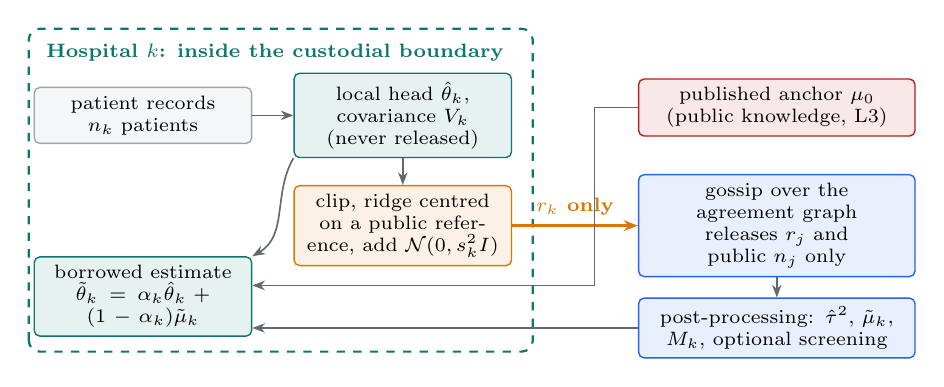
\begin{tikzpicture}[x=1cm, y=1cm, font=\scriptsize,
  blk/.style={draw=#1, fill=#1!10, line width=0.5pt, rounded corners=2pt, align=center, inner sep=3pt, text width=2.55cm},
  blk/.default=famC,
  arr/.style={-{Stealth[length=1.6mm]}, line width=0.6pt, draw=edgec},
  priv/.style={-{Stealth[length=1.8mm]}, line width=1.1pt, draw=famT}]
% hospital k
\path[draw=famC, line width=0.8pt, dashed, rounded corners=4pt] (-0.25,-3.55) rectangle (6.15,0.55);
\node[anchor=north west, font=\scriptsize\bfseries, text=famC] at (-0.15,0.48) {Hospital $k$: inside the custodial boundary};
\node[blk=grayc] (data) at (1.2,-0.55) {patient records\\ $n_k$ patients};
\node[blk] (fit) at (4.5,-0.55) {local head $\hat{\theta}_k$, covariance $V_k$\\ (never released)};
\node[blk=famT] (noise) at (4.5,-1.95) {clip, ridge centred on a public reference, add $\mathcal{N}(0,s_k^2 I)$};
\node[blk] (final) at (1.2,-2.85) {borrowed estimate\\ $\tilde{\theta}_k=\alpha_k\hat{\theta}_k+(1-\alpha_k)\tilde{\mu}_k$};
% outside
\node[blk=famE, text width=3.3cm] (net) at (9.25,-1.95) {gossip over the agreement graph\\ releases $r_j$ and public $n_j$ only};
\node[blk=famE, text width=3.3cm] (post) at (9.25,-3.25) {post-processing: $\hat{\tau}^2$, $\tilde{\mu}_k$, $M_k$, optional screening};
\node[blk=famO, text width=3.3cm] (anchor) at (9.25,-0.45) {published anchor $\mu_0$ (public knowledge, L3)};
% arrows
\draw[arr] (data) -- (fit);
\draw[arr] (fit) -- (noise);
\draw[priv] (noise.east) -- node[above, text=famT, font=\scriptsize\bfseries] {$r_k$ only} (net.west);
\draw[arr] (net) -- (post);
\draw[arr] (post.west) -- (final.east |- post.west);
\draw[arr] (anchor.west) -- ++(-0.55,0) |- ([yshift=4pt]final.east);
\draw[arr] (fit.south west) to[out=-120, in=30] (final.north east);
\end{tikzpicture}
}
\caption{The privacy boundary of GHB. Patient records and the local head stay inside the hospital. Only the hospital's masked share $r_k$ of the two network sums crosses the boundary; the masks cancel in the totals, which carry the privacy noise. Everything computed from the totals is post-processing (Proposition~\ref{prop:ghbprivacy}), and the hospital combines it with its own noise-free data locally.}
\label{fig:boundary}
\end{figure}

\begin{algorithm}[t]
\caption{Graph Hierarchical Borrowing (one round of model fitting)}\label{alg:ghb}
\KwIn{graph $\mathcal{G}$ with gossip matrix $W$; privacy budget $(\epsilon,\delta)$, i.e.\ $\rho$; feature bound $G$; public encoder $f_{\phi_0}$; optionally a published model $\mu_0$ with stated uncertainty $\sigma_0^2$, and the estimates of other networks fitting the same head}
\ForEach{hospital $k$ in parallel}{
 adapt $f_{\phi_0}$ to local unlabeled data with adapters (L1)\;
 compute $\sum_{i\in k}x_i(y_i-\tfrac12)$ and $\sum_{i\in k}x_ix_i^{\top}/4$ (its diagonal alone if $s_J\sqrt{p}>NG^2/(4p)$); add pairwise masks agreed with neighbours and a share $\mathcal{N}(0,s^2/K)$ of the noise, $s_S=2G/\sqrt{\rho}$, $s_J=\sqrt2\,G^2/(4\sqrt{\rho})$\tcp*{the only released quantities}
}
gossip the masked shares until consensus: every hospital obtains $\tilde{S}$ and $\tilde{J}$ (Proposition~\ref{prop:gossip})\tcp*{the masks cancel}
compute $\hat{w}=A\tilde{S}$ and $V_{\mathrm{dp}}=s_S^2AA^{\top}$, $A=(\tilde{J}^{+}+I/s_0^2)^{-1}$; shrink $\hat{w}$ toward other networks' estimates, and combine it with $\mu_0$ unless they conflict\tcp*{post-processing}
\ForEach{hospital $k$}{
 compute locally $s_k$ at $\hat{w}$ and $J_k$; leave-one-out estimate $\mu_{-k}=\hat{w}-H_{-k}^{-1}s_k$, $V_{-k}=H_{-k}^{-1}+V_{\mathrm{dp}}$\;
 fit the local head under each prior $\mathcal{N}(\mu_{-k},\mathrm{diag}(\tau_q^2)+s_0^2e_1e_1^{\top}+V_{-k})\cdot\mathcal{N}(0,D_s)$, $q=1,\dots,Q$, $s\in\{0.5,1,2.5\}$, and under $\mathcal{N}(0,D_s)$ alone (the intercept is not borrowed); average the fits weighted by the marginal likelihood of the local data (Remark~\ref{rem:tau}); in the Gaussian case with known $\tau^2$ this is $\tilde{\theta}_k=\alpha_k^{\star}\hat{\theta}_k+(1-\alpha_k^{\star})\tilde{\mu}_k$ with $\alpha_k^{\star}$ of Proposition~\ref{prop:borrowing}\;
 calibrate with conformal prediction on local held-out data (L4); rank unlabeled patients by posterior variance (L5)\;
}
\end{algorithm}

\begin{proposition}[Privacy of GHB]\label{prop:ghbprivacy}
Suppose every patient's features satisfy $\|x\|\le G$, the secure summation reveals only the two totals, and the noise of each total has the stated variance. Then the pair $(\tilde{S},\tilde{J})$ satisfies $\rho$-zero-concentrated differential privacy, and hence $(\epsilon,\delta)$-differential privacy with $\epsilon=\rho+2\sqrt{\rho\ln(1/\delta)}$, with respect to replacing the record of any one patient at any hospital. Every model, estimate and message that GHB computes afterwards satisfies the same guarantee. If $c$ of the $K$ hospitals collude and remove their own noise shares from the totals, the guarantee for the other hospitals' patients weakens to $\rho K/(K-c)$.
\end{proposition}
\begin{proof}
Replacing one record changes $\sum\psi_i$ by at most $2G$ and the upper triangle of $\sum\phi_i$, or its diagonal, by at most $\sqrt2\,G^2/4$ in $\ell_2$ norm, as shown above; whether the diagonal or the full matrix is released depends only on public quantities. The Gaussian mechanism with noise $s$ and sensitivity $\Delta$ is $\Delta^2/(2s^2)$-zCDP \cite{bun2016concentrated}, which is $\rho/2$ for each total; zCDP composes additively, so the pair is $\rho$-zCDP, and the conversion to $(\epsilon,\delta)$ is that of \citet{bun2016concentrated}. Everything computed afterwards is a function of the two totals, of public quantities, and, at hospital $k$, of hospital $k$'s own data used only inside it and never released, so post-processing \cite{dwork2014algorithmic} gives the second claim; the networks' exchange of their estimates and the gossip of the masked shares are post-processing as well. Colluders who subtract their shares leave noise of variance $s^2(K-c)/K$, for which the same computation gives $\rho K/(K-c)$.
\end{proof}

A hospital's final model uses its own data without noise and is therefore not private; like the local estimate in Proposition~\ref{prop:borrowing}, it never leaves the hospital. GHB-lite satisfies the same guarantee per hospital with no trust in summation. None of GHB's ingredients is new: shrinkage dominates separate estimation \cite{efron1973steins,stein1956inadmissibility}, noise on sums is the cheapest privacy \cite{bonawitz2017practical,dwork2014algorithmic}, gossip removes the server \cite{boyd2006randomized}, evidence weighting lets borrowing switch itself off, and shared representations keep the head small \cite{maurer2016benefit,tripuraneni2020theory}. Its case is that it is the simplest combination that meets all five requirements; the next two sections test whether it also performs.

%% EXPERIMENTS
%% ===================================================================
\section{Experiments}\label{sec:experiments}

The propositions assume $\tau^2$ and $M$ known, a Gaussian model and honest participants. Eighteen Monte Carlo simulations, where the truth is known, measure what is lost when each assumption fails; Section~\ref{sec:real} then asks the same of real hospitals. Figure~\ref{fig:sim-forest} places every scenario on one axis and Table~\ref{tab:sims} lists questions and answers; the supplement gives each design in full.

\subsection{Design of the simulation study}\label{sec:sim-design}

Unless stated otherwise the network has 24 hospitals of 16 to 479 patients (log-normal, median 100), $\sigma^2=1$, $C=1$, $\epsilon=1$, $\delta=10^{-5}$, and releases are averaged by 60 gossip rounds on the ring with two-hop links of Figure~\ref{fig:gossip}. Errors are relative to local estimation, so values below 1 mean that hospitals gain. The simulations were built for GHB-lite, whose theory is that of Section~\ref{sec:model}; GHB was added to the logistic comparisons (Simulations 8, 10, 11 and 15) without changing anything else. These worlds favour GHB-lite on purpose: its public feature distribution is exactly that of every hospital, and 24 hospitals of about a hundred patients make its releases informative enough to learn $\tau$. Every baseline spends the same budget under zero-concentrated accounting, and its hyperparameters are tuned on separate replicates with access to the true loss, which no deployment has; GHB and GHB-lite tune nothing. Results are means with $\pm2$ standard errors.

\begin{figure}[t]
\centering
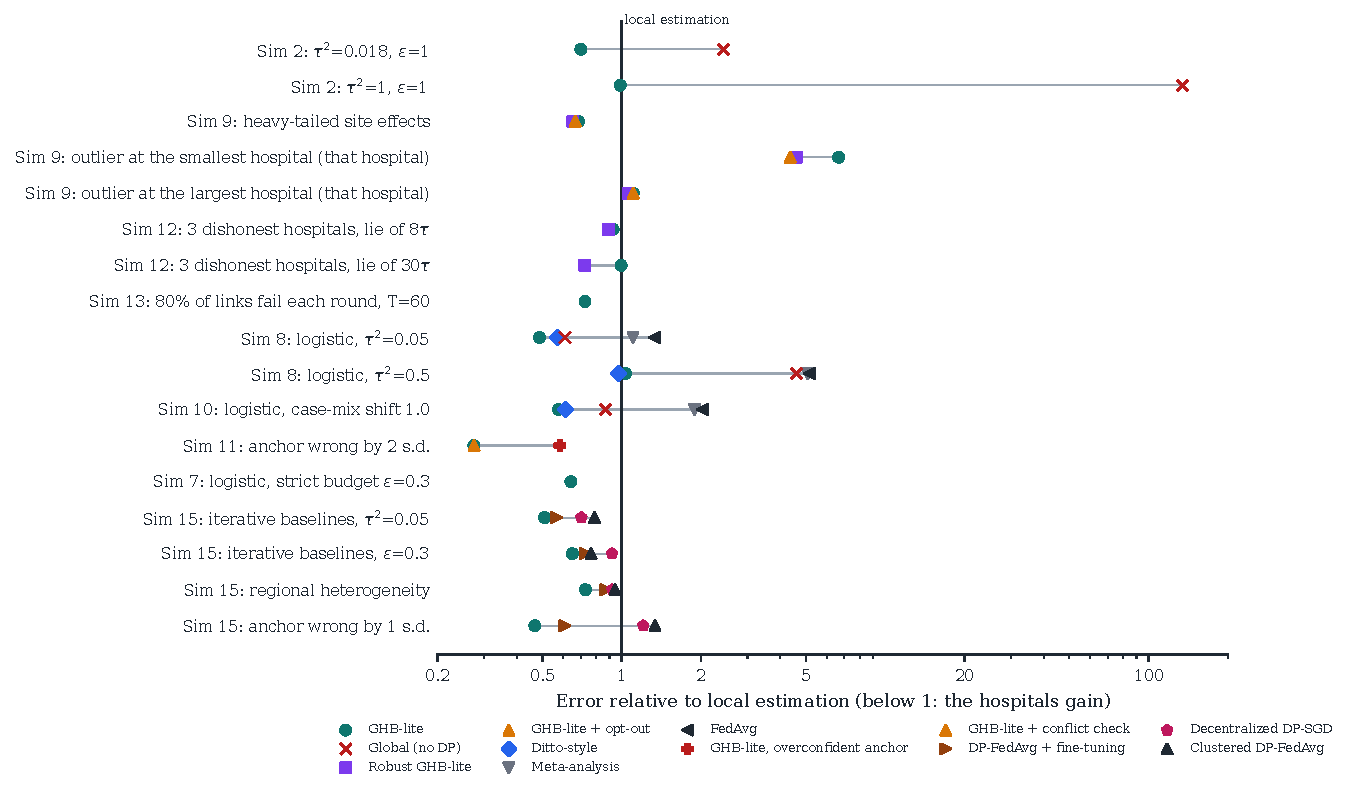
\includegraphics[width=\linewidth]{supplement/figures/sim_forest}
\caption{Summary of Simulations 2 to 15. Each row is a scenario and each marker a method; the horizontal position is the method's error relative to local estimation (mean risk $R_k/v_k$ in the Gaussian simulations, mean excess log-loss divided by that of local estimation in the logistic ones). Left of the vertical line, the hospitals gain. Rows marked ``that hospital'' report the outlying hospital alone.}
\label{fig:sim-forest}
\end{figure}
\begin{table}[t]
\caption{The eighteen simulations, the held-out real networks, and their main results. The simulations run GHB-lite; where GHB was added, its value follows (``GHB''). Relative risk is $R_k/v_k$ and logistic results are mean excess log-loss (nats); below the local value, hospitals gain. $\epsilon=1$ unless stated.}
\label{tab:sims}
\scriptsize
\begin{tabularx}{\linewidth}{@{}>{\raggedright\arraybackslash}p{2.2cm}>{\raggedright\arraybackslash}p{3.3cm}X@{}}
\toprule
Simulation & Question & Result\\
\midrule
1 Closed forms & Do Propositions~\ref{prop:borrowing} and~\ref{prop:privatized} match simulation? & \SimOneWithin{} of \SimOneChecks{} comparisons within two standard errors; largest relative deviation \SimOneMaxRel\\
2 Heterogeneity & Is plug-in GHB-lite ever worse than local estimation? & Worst hospital at most \SimTwoWorstGHB{} for $\tau^2\in[10^{-4},1]$; a global model reaches \SimTwoWorstPool\\
3 Equity, network size & Who gains, and how many hospitals are needed? & Gain in $n^{\eff}$ \SimThreeSmall{} for small, \SimThreeLarge{} for large hospitals; with 3 hospitals relative risk \SimThreeKThreeDL{} against \SimThreeKThreeOracle{} with known $\tau^2$\\
4 Gossip rounds & How many rounds are needed? & Within 2\% of exact averaging after \SimFourRandomTwo{} to \SimFourRingTwo{} rounds, against \SimFourRandomPred{} to \SimFourRingPred{} from the worst-case bound\\
5 Joint release & Does secure aggregation among small hospitals help? & Only if all hospitals are small: $B$ from \SimFiveSmallGOneEpsTenth{} to \SimFiveSmallGEightEpsTenth{} at $\epsilon=0.1$; from \SimFiveMixedGOneEpsTenth{} to \SimFiveMixedGEightEpsTenth{} in a mixed network\\
6 Regional structure & When does the GMRF prior of Equation~\eqref{eq:gmrf} pay off? & Worse when regions barely differ (\SimSixGMRFLow{} against \SimSixGHBLow), far better when they differ (\SimSixGMRFHigh{} against \SimSixGHBHigh)\\
7 Logistic heads & Does it work beyond the Gaussian model? & \SimSevenLocal{} local, \SimSevenGHB{} GHB-lite, \SimSevenGlobal{} pooled without privacy; \SimSevenGHBTenth{} against \SimSevenLocalTenth{} at $\epsilon=0.3$\\
8 Federated baselines & Does it beat existing approaches at the same budget? & At $\tau^2=0.05$: GHB-lite \SimEightMidGHB, GHB \SimEightMidV, Ditto-style \cite{li2021ditto} \SimEightMidDitto, meta-analysis \SimEightMidMeta, FedAvg \cite{mcmahan2017communication} \SimEightMidFedavg; at $\tau^2=0.5$ GHB-lite \SimEightHighGHB{} against local \SimEightHighLocal\\
9 Atypical hospitals & What happens to a hospital unlike the others? & Heavy tails: \SimNineTGHB, robust prior \SimNineTRobust; an outlier at the smallest hospital loses (\SimNineSmallGHB, at best \SimNineSmallOpt), at the largest barely (\SimNineLargeGHB)\\
10 Case-mix shift & Does it survive hospitals with different patients? & Shift of one s.d.: GHB-lite \SimEightShiftGHB, GHB \SimEightShiftV, Ditto-style \cite{li2021ditto} \SimEightShiftDitto, pooled \SimEightShiftPooled, local \SimEightShiftLocal\\
11 Wrong anchor & What if the published model is wrong? & Honest uncertainty or a conflict check: at most \SimElevenHonestMax{} at any error; an overconfident anchor \SimElevenOverTwo{} at 2 s.d.; GHB at most \SimElevenVMax\\
12 Dishonest hospitals & What if hospitals lie? & Plain GHB-lite never above \SimTwelveWorstGHB; robust screening keeps \SimTwelveRobustLarge{} against large lies, at a cost of \SimTwelveRobustNone{} against \SimTwelveGHBNone{} when nobody lies\\
13 Link failures & What if links fail during gossip? & With 80\% of links failing each round, \SimThirteenEighty{} after 60 rounds against \SimThirteenExact{} with exact averaging\\
14 Repeated releases & What do refits on the same patients cost? & After \SimFourteenR{} refits, $B=\SimFourteenBasic$ with basic composition and \SimFourteenZcdp{} with zero-concentrated accounting (one release: \SimFourteenOne)\\
15 Iterative federated learning & Does it beat multi-round training with the same budget and tuned hyperparameters? & At $\tau^2=0.05$: GHB-lite \SimFifteenMidGHB, GHB \SimFifteenMidV, DP-FedAvg \cite{mcmahan2018learning} with fine-tuning \SimFifteenMidFT, decentralized DP-SGD \cite{lian2017can} \SimFifteenMidDec, clustered \SimFifteenMidClus; at $\epsilon=0.3$ GHB-lite \SimFifteenStrictGHB{} against \SimFifteenStrictFT; worst hospital at most \SimFifteenGHBWorstMax{} for GHB-lite except at $\tau^2=0.5$, \SimFifteenFTWorstMin{} to \SimFifteenFTWorstMax{} for fine-tuning\\
16 Ablation & What does each component contribute? & Error relative to GHB-lite without it: ridge release up to \SimSixteenRidgeMax; $X^\top y$ release \SimSixteenXtyShift{} under case-mix shift; plug-in $\tau^2$ up to \SimSixteenTauMeanMax{} (posterior mean) and \SimSixteenTauDLMax{} (DerSimonian-Laird \cite{dersimonian1986meta}); no conflict check \SimSixteenNoCheckAnchor{} with a wrong anchor; equal weights up to \SimSixteenEqualMax; gossip and accounting free\\
17 Sensitivity & How much do settings and conditions matter? & Settings: quantiles, public sample, threshold and rounds ($\ge 20$) flat; prior scale of $\tau$ \SimSeventeenScaleMin{} to \SimSeventeenScaleMax; misstated anchor up to \SimSeventeenAnchorSdMax. Conditions: error \SimSeventeenRelMin{} to \SimSeventeenRelMax{} of local, worst hospital at most \SimSeventeenWorstMax\\
16B, 17B GHB & Which of GHB's components and settings matter, and across which conditions? & Intercept borrowed \SimSixteenBIntMin{} to \SimSixteenBIntMax{} of GHB's error (this world shares base rates); no non-borrowing components down to \SimSixteenBSafetyMin; most settings within \SimSixteenBSmallMax; across conditions \SimSeventeenBRelMin{} to \SimSeventeenBRelMax{} of local, worst hospital at most \SimSeventeenBWorstMax\\
18 Group fairness & What does borrowing do to a protected group? & Minority excess log-loss ($\times10^{-3}$) with a shared disparity: GHB-lite \SimEighteenSharedGHBMin, local \SimEighteenSharedLocalMin, FAIR-FATE \cite{salazar2023fairfate} \SimEighteenSharedFFEQOMin; disparities that vary: GHB-lite \SimEighteenVariesGHBMin, global \SimEighteenVariesGlobalMin; equalized odds of GHB-lite within 0.02 of the true models, FAIR-FATE closer to parity\\
Real data & Does it hold on real hospitals, against the literature tuned as a consortium could? & Five held-out TCGA networks: GHB \SimTCOneGHB{} and \SimTCTenGHB{} relative to local at $\epsilon=1$ and 10; best literature method \SimTCOneFT{} and \SimTCTenDitto{} (Section~\ref{sec:real})\\
\bottomrule
\end{tabularx}
\end{table}

\subsection{Does the theory survive estimation?}\label{sec:sim-theory}

A real network must estimate $\tau^2$ and $M$ from privatized releases, so the first question is how much of the predicted gain survives, and for whom. Simulation 1 confirms the closed forms. Across four orders of magnitude of heterogeneity (Simulation 2, Figure~\ref{fig:sim-het}), plug-in GHB-lite stays at or below local estimation for every hospital, while a global model becomes up to \SimTwoMeanPool{} times worse on average and \SimTwoWorstPool{} times worse for its worst hospital; the price of estimating $\tau^2$ appears only when heterogeneity is tiny (\SimTwoMinGHB{} against \SimTwoMinOracle{} with the true value). Gossip is free once mixed: 11 to 35 rounds suffice on the topologies of Figure~\ref{fig:gossip} (Simulation 4), and mixing survives 80\% of links failing each round (\SimThirteenEighty{} against \SimThirteenExact, Simulation 13).

\begin{figure}[t]
\centering
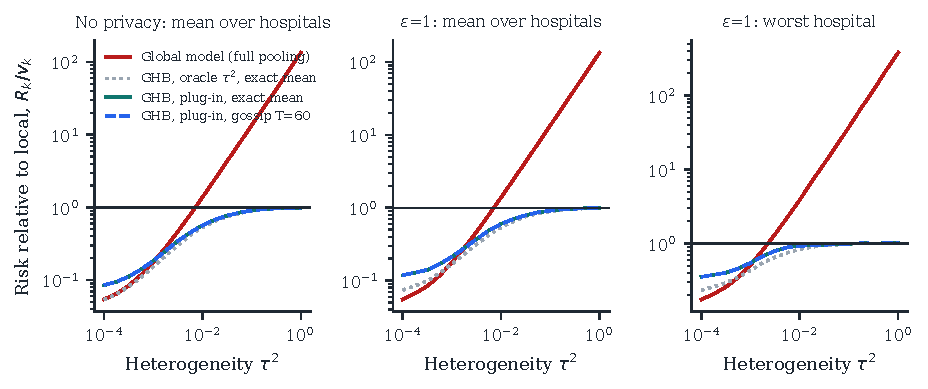
\includegraphics[width=\linewidth]{supplement/figures/s2_heterogeneity}
\caption{Simulation 2: risk relative to local estimation against heterogeneity, for 24 hospitals of 16 to 479 patients. Plug-in GHB-lite estimates $\tau^2$ and $M$ from privatized releases averaged by gossip; the oracle uses the true $\tau^2$; the global model is the sample-size weighted mean of all site estimates, computed without privacy.}
\label{fig:sim-het}
\end{figure}

Who gains is what (R4) asks. Every hospital gains about $B\approx\SimThreeB$ virtual patients (Simulation 3, Figure~\ref{fig:sim-equity}), so hospitals of 60 patients or fewer multiply their effective sample size by \SimThreeSmall{} and those of 300 or more by \SimThreeLarge; a global model helps small hospitals less (\SimThreePoolSmall) and cuts large ones to \SimThreePoolLarge{} of their own. With three hospitals, $\tau^2$ is too poorly estimated and most of the gain is lost; a half-Cauchy prior helps from four upward.

\begin{figure}[t]
\centering
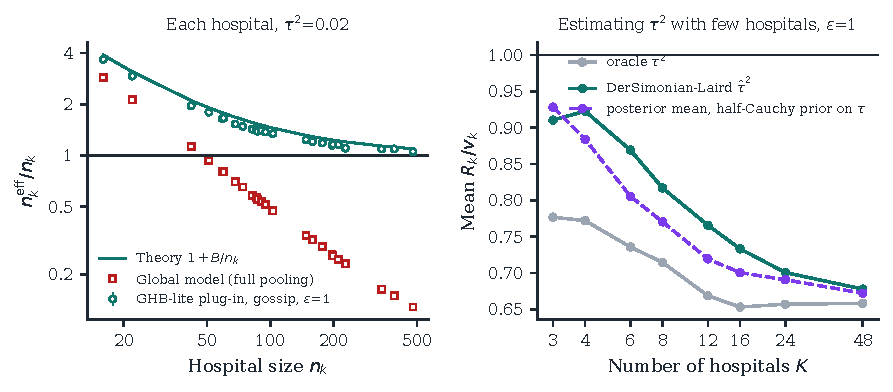
\includegraphics[width=\linewidth]{supplement/figures/s3_equity}
\caption{Simulation 3. Left: effective sample size relative to own size for each hospital at $\tau^2=0.02$, $\epsilon=1$; the line is $1+B/n_k$ from Equation~\eqref{eq:borrowed}. Right: mean relative risk against the number of hospitals for three ways of obtaining $\tau^2$.}
\label{fig:sim-equity}
\end{figure}

\subsection{Against federated and meta-analytic baselines}\label{sec:sim-baselines}

Gaining over local estimation matters only if the method also beats what a network could adopt instead. From here on the heads are logistic regressions on four features, every baseline consumes the same budget, and its hyperparameters are tuned on the true loss.

\paragraph{One-shot baselines} Simulations 8 and 10 compare methods that use the same releases (Figure~\ref{fig:sim-baselines}, Table~\ref{tab:sim8}). At $\tau^2=0.05$ GHB-lite reaches \SimEightMidGHB, below a Ditto-style \cite{li2021ditto} model tuned on separate replicates (\SimEightMidDitto) and below a global model trained on pooled data without privacy (\SimEightMidPooled); federated averaging \cite{mcmahan2017communication} and meta-analysis, which give every hospital one model, are worse than local (\SimEightMidFedavg{} and \SimEightMidMeta{} against \SimEightMidLocal). Under case-mix shift GHB-lite keeps its lead (\SimEightShiftGHB{} against \SimEightShiftDitto). From $\tau^2=0.2$ the tuned Ditto-style model is slightly better, and at $\tau^2=0.5$ it is the only method that gains. GHB is less accurate than GHB-lite here (\SimEightMidV{} at $\tau^2=0.05$), for two reasons that are this world's: it cannot learn $\tau$ from per-hospital releases, and these hospitals differ in base rate no more than in slopes, so not borrowing the intercept costs rather than protects.

\begin{figure}[t]
\centering
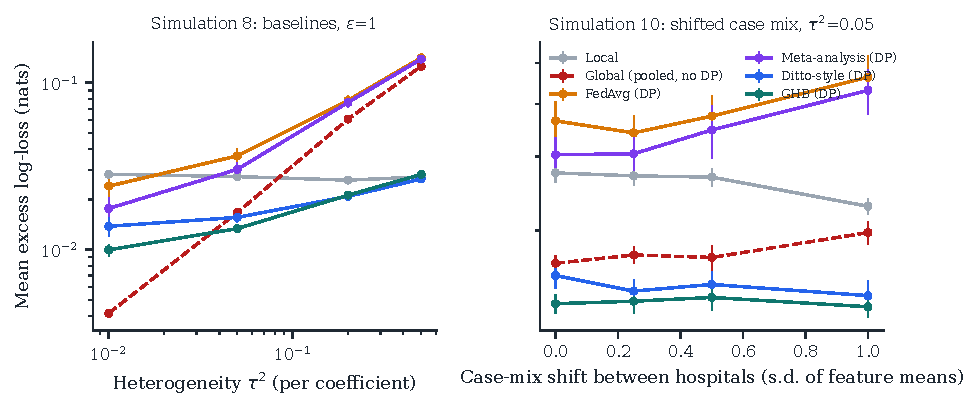
\includegraphics[width=\linewidth]{supplement/figures/sim8_baselines}
\caption{Simulations 8 and 10, logistic-regression heads. Mean excess log-loss over the true model of GHB-lite, of private baselines that use the same releases (one-shot federated averaging \cite{mcmahan2017communication}, random-effects meta-analysis, Ditto-style \cite{li2021ditto} personalization tuned on separate replicates) and of a global model trained on the pooled data without privacy. Left: against coefficient heterogeneity. Right: against case-mix shift between hospitals at $\tau^2=0.05$. Bars: $\pm 2$ standard errors.}
\label{fig:sim-baselines}
\end{figure}
\begin{table}[t]
\caption{Simulations 8 and 10: exact values behind Figure~\ref{fig:sim-baselines}. Values are mean excess log-loss in $10^{-3}$ nats, with two Monte Carlo standard errors in grey; the lowest private method in each row is bold. All private methods use the same releases at $\epsilon=1$; the pooled model uses no privacy. GHB (joint releases) appears in the table but not in the figure.}
\label{tab:sim8}
\scriptsize
\setlength{\tabcolsep}{4pt}
\begin{tabular}{@{}lrrrrrrr@{}}
\toprule
Setting & Local & GHB & GHB-lite & \makecell[r]{Ditto-style\\\cite{li2021ditto}} & \makecell[r]{Meta-analysis\\\cite{dersimonian1986meta}} & \makecell[r]{FedAvg\\\cite{mcmahan2017communication}} & Pooled, no DP\\
\midrule
\csname @@input\endcsname../Collectively_Big_Locally_Small/supplement/results/tables/t_sim8.tex 
\bottomrule
\end{tabular}
\end{table}

\paragraph{Iterative federated learning} Simulation 15 faces multi-round training: DP-FedAvg \cite{mcmahan2017communication,mcmahan2018learning} with and without fine-tuning, decentralized DP-SGD \cite{lian2017can} on the same graph, and clustered training in the style of IFCA \cite{ghosh2020efficient}, all tuned on \SimFifteenTune{} replicates with the true loss (Figure~\ref{fig:sim-literature}, Tables~\ref{tab:sim15} and~\ref{tab:sim15worst}); four of the ten settings were held out while GHB-lite was designed. GHB-lite is the most accurate method in six settings, three of them held out, for instance at $\tau^2=0.05$ (\SimFifteenMidGHB{} against \SimFifteenMidFT{} for DP-FedAvg with fine-tuning) and at $\epsilon=0.3$ (\SimFifteenStrictGHB{} against \SimFifteenStrictFT); the tuned Ditto-style model is slightly better at $\tau^2=0.2$, without privacy and with a wrong anchor, and at $\tau^2=0.5$ nothing beats local estimation. Its gain at a strict budget comes from borrowing, not the anchor: a tuned local control started from the anchor reaches \SimFifteenStrictAnchorGD{} and becomes worse than local when the anchor is wrong (\SimFifteenAnchorAnchorGD). GHB, with joint releases, does less well in this world, whose hospitals share their base rates: significantly better than local estimation in \SimStSimLocBetter{} of \SimStSimLocN{} settings, but worse than the tuned Ditto-style model in \SimStSimDittoWorse{} and than DP-FedAvg with fine-tuning in \SimStSimFTWorse{} (supplement).

The methods differ most in who pays. GHB-lite's worst hospital stays within a factor \SimFifteenGHBWorstMax{} of its local error in every private setting except $\tau^2=0.5$; fine-tuning leaves some hospital \SimFifteenFTWorstMin{} to \SimFifteenFTWorstMax{} times worse off, usually a large one whose data the federated model overrides (the eight largest go from \SimFifteenStrictLocalLarge{} alone to \SimFifteenStrictFTLarge{} at $\epsilon=0.3$, against \SimFifteenStrictGHBLarge{} with GHB-lite). What remains is the cost of not knowing $\tau^2$: with the true value GHB-lite would reach \SimFifteenStrictOracle{} at $\epsilon=0.3$. GHB, for the reasons above, beats every iterative baseline in \SimFifteenVBeatsIter{} of the ten settings and trails GHB-lite in all ten (\SimFifteenMidV{} at $\tau^2=0.05$), with its worst hospital within a factor \SimFifteenVWorstMax{} of its local error. In worlds where GHB-lite's inversion is exact, per-hospital releases are worth their noise; Section~\ref{sec:real} shows that on real hospitals they were not.

\begin{figure}[t]
\centering
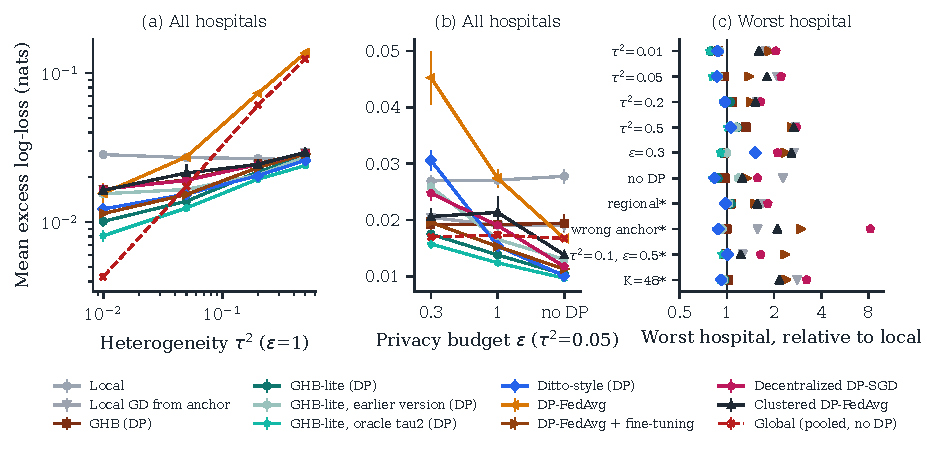
\includegraphics[width=\linewidth]{supplement/figures/sim15_literature}
\caption{Simulation 15: GHB-lite against iterative federated learning at the same privacy budget (logistic heads, 24 hospitals, mean excess log-loss over \SimFifteenReps{} replicates, $\pm2$ standard errors). Baseline hyperparameters are tuned with access to the true loss; GHB-lite is not tuned. (a) Against heterogeneity at $\epsilon=1$. (b) Against the privacy budget at $\tau^2=0.05$. (c) The worst hospital's error relative to its own local estimate in each setting; right of 1, some hospital is worse off than alone; settings marked $\ast$ were held out while GHB-lite was designed. ``GHB-lite, earlier version'' is an earlier formulation that released ridge fits, shown for reference; ``GHB-lite, oracle $\tau^2$'' uses the true heterogeneity and is a reference, not a method.}
\label{fig:sim-literature}
\end{figure}
\begin{table}[t]
\caption{Simulation 15: exact values behind Figure~\ref{fig:sim-literature}. Values are mean excess log-loss in $10^{-3}$ nats, with two Monte Carlo standard errors in grey; the lowest private method in each row is bold. Settings marked $\ast$ were held out while GHB-lite was designed. FT: fine-tuning \cite{mcmahan2018learning}. The figure's marker labelled GHB is GHB-lite; GHB (joint releases) appears in the table.}
\label{tab:sim15}
\scriptsize
\setlength{\tabcolsep}{2.2pt}
\resizebox{\linewidth}{!}{\begin{tabular}{@{}lrrrrrrrrrr@{}}
\toprule
Setting & Local & \makecell[r]{Anchor\\GD} & GHB & GHB-lite & \makecell[r]{Ditto-\\style\\\cite{li2021ditto}} & \makecell[r]{DP-FedAvg\\+ FT\\\cite{mcmahan2018learning}} & \makecell[r]{Decentr.\\DP-SGD\\\cite{lian2017can}} & \makecell[r]{Clustered\\DP-FedAvg\\\cite{ghosh2020efficient}} & \makecell[r]{GHB-lite,\\true $\tau^2$} & \makecell[r]{Pooled,\\no DP}\\
\midrule
\csname @@input\endcsname../Collectively_Big_Locally_Small/supplement/results/tables/t_sim15_mean.tex 
\bottomrule
\end{tabular}}
\end{table}
\begin{table}[t]
\caption{Simulation 15: who pays. Left: the largest ratio of any hospital's mean excess log-loss to its own local value (above 1, some hospital is worse off than alone; lowest in bold). Middle: the percentage of hospitals that gain over local estimation. Right: the mean excess log-loss of the eight largest hospitals ($10^{-3}$ nats).}
\label{tab:sim15worst}
\scriptsize
\setlength{\tabcolsep}{2.4pt}
\resizebox{\linewidth}{!}{\begin{tabular}{@{}lrrrrrrrrrrrrrr@{}}
\toprule
 & \multicolumn{8}{c}{Worst hospital, relative to local} & \multicolumn{3}{c}{Hospitals that gain (\%)} & \multicolumn{3}{c}{Eight largest}\\
\cmidrule(lr){2-9}\cmidrule(lr){10-12}\cmidrule(l){13-15}
Setting & Local & \makecell[r]{Anchor\\GD} & GHB & GHB-lite & \makecell[r]{Ditto\\\cite{li2021ditto}} & \makecell[r]{FedAvg\\+ FT\\\cite{mcmahan2018learning}} & \makecell[r]{Decentr.\\\cite{lian2017can}} & \makecell[r]{Clust.\\\cite{ghosh2020efficient}} & GHB-lite & \makecell[r]{Ditto\\\cite{li2021ditto}} & \makecell[r]{FedAvg\\+ FT\\\cite{mcmahan2018learning}} & Local & GHB-lite & \makecell[r]{FedAvg\\+ FT\\\cite{mcmahan2018learning}}\\
\midrule
\csname @@input\endcsname../Collectively_Big_Locally_Small/supplement/results/tables/t_sim15_worst.tex 
\bottomrule
\end{tabular}}
\end{table}

\paragraph{Privacy is the binding constraint} GHB-lite cuts the excess log-loss of local estimation by \SimSevenReduction{} at $\epsilon=1$ and keeps most of that at $\epsilon=0.3$ (\SimSevenGHBTenth{} against \SimSevenLocalTenth, Simulation 7), whereas releasing ridge fits instead of scores kept almost none (\SimFifteenStrictOld): what a hospital releases matters as much as how much privacy it spends. Joint release among groups of small hospitals helps only when every hospital is small (Simulation 5), and refits are affordable only under zero-concentrated accounting: after \SimFourteenR{} refits a hospital keeps $B=\SimFourteenZcdp$ virtual patients, against \SimFourteenBasic{} under basic composition (Simulation 14).

\subsection{What breaks it}\label{sec:sim-attacks}

Next, failures on purpose. \emph{Atypical hospitals} (Simulation 9) are the failure Proposition~\ref{prop:borrowing} predicts. Heavy-tailed effects keep the mean risk low (\SimNineTGHB; \SimNineTRobust{} with a Student-$t$ prior), and an outlying large hospital barely loses (\SimNineLargeGHB), but an outlying small one loses badly (\SimNineSmallGHB{} times its local risk, at best \SimNineSmallOpt{} with any safeguard): a small hospital cannot tell from its own data that it is atypical, and only external structure (Simulation 6, Equation~\eqref{eq:gmrf}) can. \emph{A wrong anchor} (Simulation 11) is harmless when its uncertainty is stated honestly or it is dropped on conflict (at most \SimElevenHonestMax), but an overconfident anchor two standard deviations off raises the error to \SimElevenOverTwo; GHB stays at or below \SimElevenVMax{} at every error. The conflict check is therefore part of both protocols. \emph{Dishonest hospitals} (Simulation 12) never pushed honest ones below local performance: a large lie inflates $\hat{\tau}^2$ and switches borrowing off (worst \SimTwelveWorstGHB), and screening releases keeps the gain against large lies (\SimTwelveRobustLarge) at a small cost when nobody lies.

\subsection{Which components and settings matter}\label{sec:sim-components}

Simulation 16 removes one component of GHB-lite at a time, on the same data and noise (Figure~\ref{fig:sim-ablation}, Table~\ref{tab:sim16}). Every component earns its place somewhere and costs little elsewhere. Releasing a ridge fit instead of the score is worse in seven of eight settings, by up to \SimSixteenRidgeMax; releasing $X^\top y$ is \SimSixteenXtyShift{} times worse under case-mix shift, which the score at the anchor absorbs; inverse-variance weighting is worth up to \SimSixteenEqualMax, the anchor up to \SimSixteenNoAnchorMax, and the conflict check \SimSixteenNoCheckAnchor{} when the anchor is wrong. The rule for $\tau$ is the most delicate: plug-in rules win slightly when hospitals are alike and lose by up to \SimSixteenTauMeanMax{} (posterior mean) or \SimSixteenTauDLMax{} (DerSimonian-Laird \cite{dersimonian1986meta}) elsewhere, while integrating $\tau$ out with each hospital's evidence is within 4\% of the best rule everywhere. Gossip and zero-concentrated accounting cost nothing for a single release.

\begin{figure}[t]
\centering
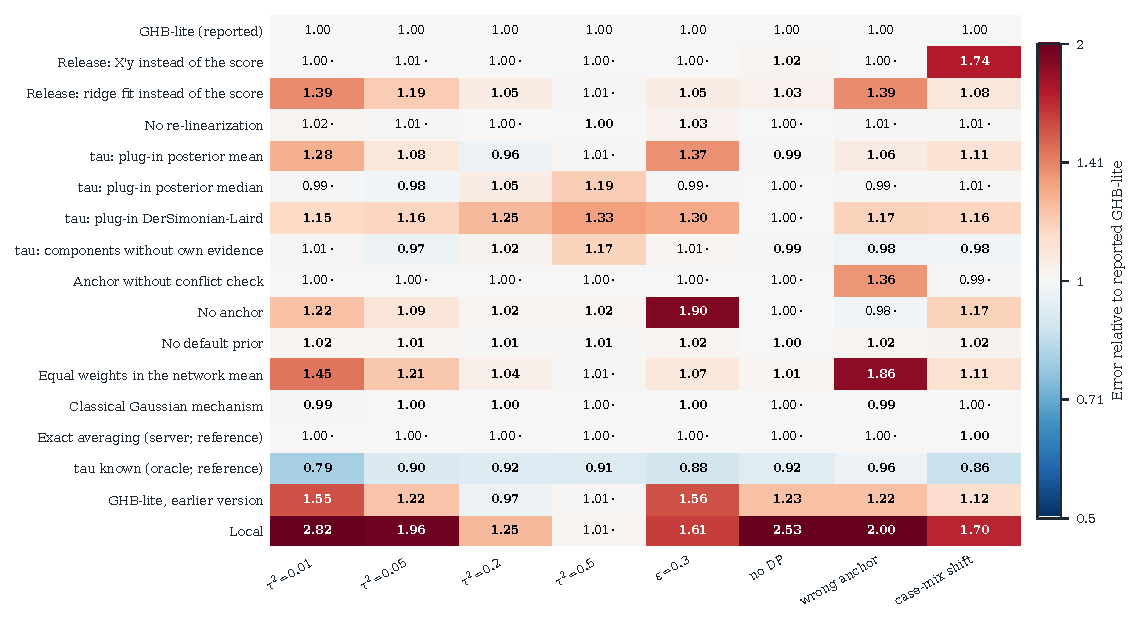
\includegraphics[width=\linewidth]{supplement/figures/sim16_ablation}
\caption{Simulation 16: ablation of GHB-lite (logistic heads, 24 hospitals, \SimSixteenReps{} replicates per setting). Each cell is the mean excess log-loss of a variant divided by that of GHB-lite as reported, computed on the same data and noise; above 1 (red), removing or replacing the component hurts. Bold: paired difference larger than two standard errors; a trailing dot marks differences within Monte Carlo error. The last three rows are references.}
\label{fig:sim-ablation}
\end{figure}
\begin{table}[t]
\caption{Simulation 16: exact values behind Figure~\ref{fig:sim-ablation}. First row: mean excess log-loss of GHB-lite as reported ($10^{-3}$ nats). Other rows: the mean excess log-loss of each variant divided by that of GHB-lite on the same data and noise (\SimSixteenReps{} replicates per setting); bold where the paired difference exceeds two standard errors. The last rows are references.}
\label{tab:sim16}
\scriptsize
\setlength{\tabcolsep}{3pt}
\begin{tabular}{@{}lrrrrrrrr@{}}
\toprule
Variant & $\tau^2=0.01$ & $\tau^2=0.05$ & $\tau^2=0.2$ & $\tau^2=0.5$ & $\epsilon=0.3$ & no DP & \makecell[r]{wrong\\anchor} & shift\\
\midrule
\csname @@input\endcsname../Collectively_Big_Locally_Small/supplement/results/tables/t_sim16.tex 
\bottomrule
\end{tabular}
\end{table}

Simulation 17 varies GHB-lite's own settings and the network around it (Figures~\ref{fig:sim-settings} and~\ref{fig:sim-conditions}, Tables~\ref{tab:sim17a} and~\ref{tab:sim17b}). Most settings hardly matter: the number of quantiles from three, the public sample from 2,000 draws, the conflict threshold from 2.5, gossip from 20 rounds. Two do: the half-Cauchy scale trades nearly identical against heterogeneous hospitals (\SimSeventeenScaleMin{} to \SimSeventeenScaleMax), with the default 0.5 within 11\% of the best everywhere, and an understated anchor uncertainty costs up to \SimSeventeenAnchorSdMax. Across 6 to 96 hospitals, median sizes of 25 to 400, budgets from $\epsilon=0.1$ to none, and every topology, the error stays between \SimSeventeenRelMin{} and \SimSeventeenRelMax{} of local and the worst hospital within a factor \SimSeventeenWorstMax; the gain grows with the number of hospitals and the budget, and is largest for hospitals of about 100 patients.

\begin{figure}[t]
\centering
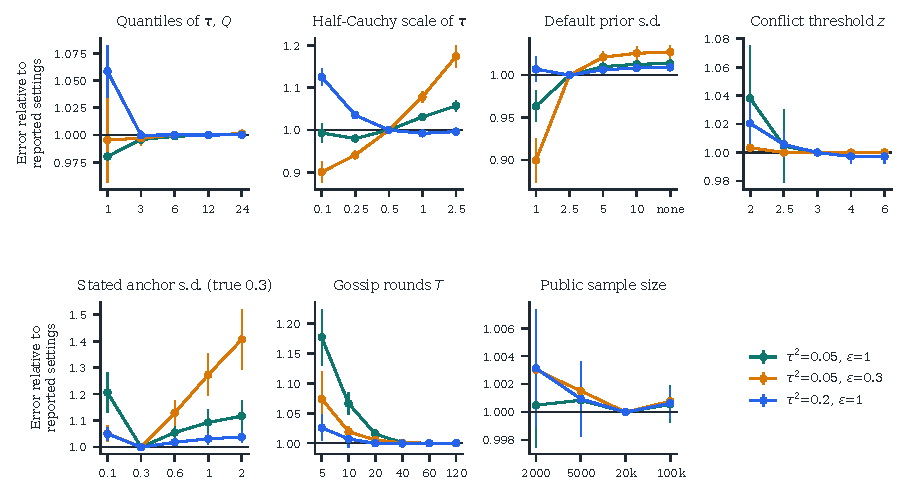
\includegraphics[width=\linewidth]{supplement/figures/sim17_settings}
\caption{Simulation 17, part A: sensitivity of GHB-lite to its own settings (logistic heads, \SimSeventeenReps{} paired replicates per point). Each point is the mean excess log-loss with the setting changed, divided by that with the reported settings ($Q=12$, scale 0.5, default prior s.d.\ 2.5, $z=3$, stated anchor s.d.\ 0.3, $T=60$, 20,000 public draws). Bars: $\pm2$ standard errors of the paired ratio.}
\label{fig:sim-settings}
\end{figure}
\begin{table}[t]
\caption{Simulation 17, part A: exact values behind Figure~\ref{fig:sim-settings}. Mean excess log-loss with one setting changed, divided by that with the reported settings (italic), on the same data and releases; two standard errors of the paired ratio in grey (\SimSeventeenReps{} replicates).}
\label{tab:sim17a}
\scriptsize
\begin{tabular}{@{}llrrr@{}}
\toprule
Setting & Value & $\tau^2=0.05$, $\epsilon=1$ & $\tau^2=0.05$, $\epsilon=0.3$ & $\tau^2=0.2$, $\epsilon=1$\\
\midrule
\csname @@input\endcsname../Collectively_Big_Locally_Small/supplement/results/tables/t_sim17_settings.tex 
\bottomrule
\end{tabular}
\end{table}
\begin{figure}[t]
\centering
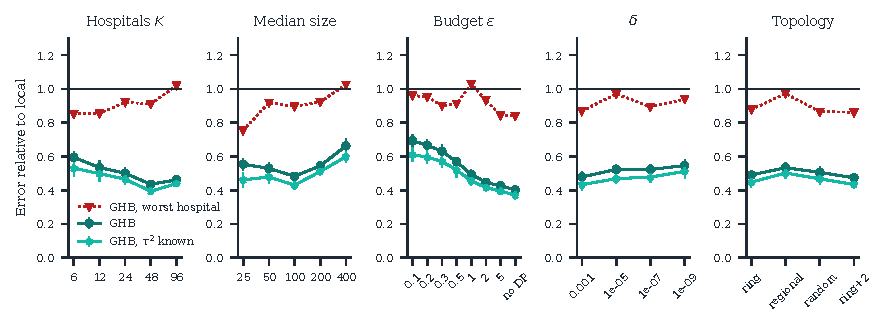
\includegraphics[width=\linewidth]{supplement/figures/sim17_conditions}
\caption{Simulation 17, part B: GHB-lite across network conditions ($\tau^2=0.05$, $\epsilon=1$, 24 hospitals of median size 100 on the ring with two-hop links unless varied; \SimSeventeenReps{} replicates per point). Mean excess log-loss relative to local estimation for GHB-lite and for GHB-lite with $\tau^2$ known ($\pm2$ standard errors), and the largest ratio of any hospital's error to its own local error (dotted).}
\label{fig:sim-conditions}
\end{figure}
\begin{table}[t]
\caption{Simulation 17, part B: exact values behind Figure~\ref{fig:sim-conditions}. Mean excess log-loss of GHB-lite relative to local estimation (two standard errors in grey), the same for GHB-lite with $\tau^2$ known, the largest ratio of any hospital's error to its own local error, and the absolute mean excess log-loss of GHB-lite and of local estimation ($10^{-3}$ nats). $\tau^2=0.05$, $\epsilon=1$, $\delta=10^{-5}$, 24 hospitals of median size 100 on the ring with two-hop links unless varied.}
\label{tab:sim17b}
\scriptsize
\begin{tabular}{@{}llrrrrr@{}}
\toprule
Condition & Value & GHB-lite / local & \makecell[r]{GHB-lite, $\tau^2$ known\\/ local} & Worst hospital & GHB-lite & Local\\
\midrule
\csname @@input\endcsname../Collectively_Big_Locally_Small/supplement/results/tables/t_sim17_conditions.tex 
\bottomrule
\end{tabular}
\end{table}

\paragraph{The same analysis for GHB} Simulation 16B repeats the ablation and sensitivity analysis for GHB in the same settings, on paired data and noise (Figure~\ref{fig:sim-ghb-ablation}; \SimSixteenBReps{} replicates per setting; supplement). In this world, which rewards borrowing, GHB's cautious choices cost what they protect against on real hospitals: borrowing the intercept would lower its error to as little as \SimSixteenBIntMin{} of the released version's, dropping the non-borrowing components to \SimSixteenBSafetyMin, and a wider prior on $\tau$ raises it by up to \SimSixteenBScaleTwoMax; the other components and settings move it by about \SimSixteenBSmallMax{} or less. Across the conditions of Simulation 17 its error stays between \SimSeventeenBRelMin{} and \SimSeventeenBRelMax{} of local estimation, with its worst hospital within a factor \SimSeventeenBWorstMax, always behind GHB-lite in this world. Section~\ref{sec:real-tcga} shows which choices pay on real hospitals.

\begin{figure}[t]
\centering
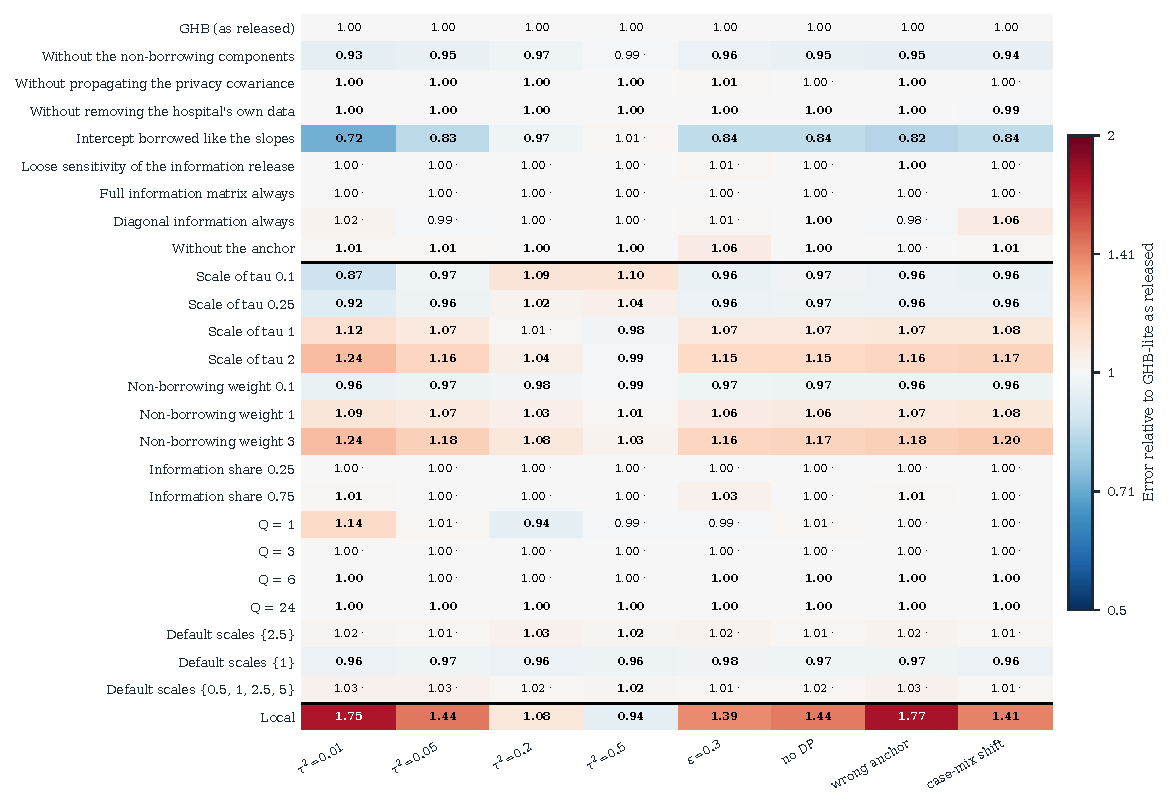
\includegraphics[width=\linewidth]{supplement/figures/sim16_ghb}
\caption{Simulation 16B: ablation (top block) and sensitivity (middle block) of GHB as released (logistic heads, 24 hospitals, \SimSixteenBReps{} replicates per setting). Each cell is the mean excess log-loss of a variant divided by that of GHB on the same data and noise; above 1 (red), the change hurts. Bold: paired difference larger than two standard errors; a trailing dot marks differences within Monte Carlo error. Last row: local estimation, a reference.}
\label{fig:sim-ghb-ablation}
\end{figure}

\subsection{Fairness to groups of patients}\label{sec:sim-fairness}

Every simulation so far asks whether some hospital pays for the others; the last asks whether some group of patients does. In Simulation 18 one feature becomes a protected attribute $S$ whose share varies across hospitals, and its coefficient is each hospital's true disparity, shared, varying, rare or of either sign across hospitals. A variant, \emph{GHB-lite, $S$ local}, keeps the disparity coefficient unborrowed at no privacy cost. FAIR-FATE \cite{salazar2023fairfate}, with its paper's settings, and federated averaging are references: both use a server, FAIR-FATE also a labelled validation set, and neither is private (Figure~\ref{fig:sim-fairness}, Table~\ref{tab:sim18}).

GHB-lite or its variant is the most accurate private method for the minority in every scenario, and the most accurate of all methods whenever hospitals disagree about the disparity. It roughly halves the minority's excess log-loss of local estimation when the disparity is shared (\SimEighteenSharedGHBMin{} against \SimEighteenSharedLocalMin{} $\times10^{-3}$ nats); when disparities vary, single models fit the minority badly (global \SimEighteenVariesGlobalMin, FAIR-FATE \SimEighteenVariesFFEQOMin) while GHB-lite reaches \SimEighteenVariesGHBMin. Because it learns $\tau$ coefficient by coefficient, GHB-lite borrows a disparity hospitals agree on and barely borrows one they disagree on, so keeping it local is a safeguard, not a default. GHB-lite leaves fairness ratios where the true models put them (within 0.02), while FAIR-FATE moves them toward parity, which, when the disparity is real, distorts the minority's predicted risks (\SimEighteenSharedFFEQOMin{} against \SimEighteenSharedGHBMin). Calibrated personalized risk and parity of decisions are different goals, and the choice belongs to the deployment.

\begin{figure}[t]
\centering
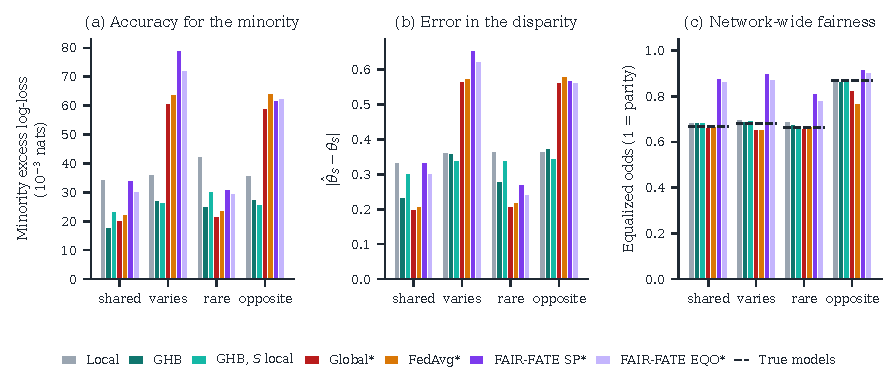
\includegraphics[width=\linewidth]{supplement/figures/sim18_fairness}
\caption{Simulation 18: a protected attribute $S$ ($\epsilon=1$, 24 hospitals, \SimEighteenReps{} replicates per scenario). (a) Mean excess log-loss of the minority group. (b) Mean absolute error of the estimated disparity, the coefficient of $S$. (c) Equalized odds of the network's decisions at threshold 0.5 (1 is parity); dashed: the true models. $\ast$: not private, with a server; FAIR-FATE \cite{salazar2023fairfate} also uses a labelled validation set at the server.}
\label{fig:sim-fairness}
\end{figure}
\begin{table}[t]
\caption{Simulation 18: exact values behind Figure~\ref{fig:sim-fairness} (\SimEighteenReps{} replicates per scenario). Mean excess log-loss over all patients, the minority ($S=1$) and the majority ($10^{-3}$ nats; two standard errors in grey); mean absolute error of the estimated disparity $|\hat\theta_S-\theta_S|$; mean absolute calibration bias in the minority, $|\mathrm{mean}(\hat p-p\mid S=1)|$ (percentage points); the largest ratio of any hospital's excess log-loss to its local one (Worst); and the statistical parity, equal opportunity and equalized odds ratios of the network's decisions at threshold 0.5 (1 is parity). Bold: best of the private methods. $\dagger$: not private, one model trained with a server. FAIR-FATE follows Algorithm~1 of \cite{salazar2023fairfate}: a third of the hospitals per round, 10 local epochs of mini-batch gradient descent (batches of 10, learning rate 0.01), $\lambda_0=0.5$, $\rho=0.05$, $\mathrm{MAX}=0.9$, $\beta_0=0.9$, 100 rounds, and a labelled validation set of a fifth of all patients at the server; federated averaging \cite{mcmahan2017communication} uses the same protocol without the fairness update. All federated models start from the anchor $\mu_0$.}
\label{tab:sim18}
\scriptsize
\setlength{\tabcolsep}{3pt}
\begin{tabular}{@{}lllrrrrrrr@{}}
\toprule
 & \multicolumn{3}{c}{Excess log-loss} & & & & \multicolumn{3}{c}{Fairness of decisions}\\
\cmidrule(lr){2-4}\cmidrule(l){8-10}
Method & All & Minority & Majority & $|\hat\theta_S-\theta_S|$ & \makecell[r]{Calib.\\bias} & Worst & SP & EO & EQO\\
\midrule
\csname @@input\endcsname../Collectively_Big_Locally_Small/supplement/results/tables/t_sim18.tex 
\bottomrule
\end{tabular}
\end{table}


%% REAL DATA
%% ===================================================================
\section{Real Hospital Networks}\label{sec:real}

The simulations control everything; real data control nothing. This section asks whether GHB's advantages survive real hospitals, real heterogeneity and real sample sizes, against the federated and personalized methods that apply, at the same privacy budget. It reports two studies. The first is a confirmation on networks that no part of GHB's development had seen. Its rule, its predictions and the frozen configuration of every method were committed to the repository before it ran (Section~\ref{sec:real-tcga}). The second is the earlier benchmark of eight smaller networks, on which GHB-lite was developed and its limits were found (Section~\ref{sec:real-eight}). The design of GHB in Section~\ref{sec:logit} came out of those limits, and every step of that development is reported, including the two pre-registered attempts that failed.

\subsection{A pre-registered test on unseen networks}\label{sec:real-tcga}

\paragraph{Networks and model} The Cancer Genome Atlas \cite{weinstein2013cancer,grossman2016toward} records, for every patient, the institution that contributed the tissue. Each cancer type is a network, and each institution with at least five eligible patients is a hospital. The outcome is death within two years of diagnosis; patients alive with less than two years of follow-up are excluded. Every hospital fits a logistic regression with eight coefficients: intercept, age, sex, pathologic stage III, stage IV, tumour stage T3 or T4, nodal involvement and a prior malignancy, with $\|x\|\le\sqrt{8}$ by construction (FIGO stage replaces the AJCC stage for the gynecologic cancers). Twelve networks served for development: lung squamous and adenocarcinoma, head and neck, bladder, stomach, liver, clear-cell and papillary kidney, colon, rectum, pancreas and oesophagus (5 to 17 hospitals each). The confirmation set was then fixed by a rule on counts alone, before any model was fitted to it. It contains every further TCGA project with at least four such hospitals and at least fifteen deaths: breast (8 hospitals), mesothelioma (9), ovarian (15), endometrial (15) and uterine carcinosarcoma (5). Hospitals hold 5 to 109 eligible patients.

\paragraph{Protocol} Every hospital is evaluated on its own held-out patients by ten repetitions of stratified five-fold cross-validation, and errors are held-out log-loss relative to local estimation under the default prior $\mathcal{N}(0,2.5^2)$. Every private method spends the same budget, $\epsilon\in\{1,10\}$ with $\delta=10^{-5}$ under zero-concentrated accounting. The literature methods are DP-FedAvg with local fine-tuning, with and without secure aggregation; clustered DP-FedAvg; APFL; Ditto \cite{li2021ditto}; and pFedMe \cite{tdinh2020personalized}. Each has a grid of 18 to 54 configurations, and how it is tuned decides how it compares. In the \emph{realistic} arm, each method uses the configuration with the lowest mean error over the twelve development networks, frozen before the confirmation. This is what a consortium could do with networks it already has. In the \emph{oracle} arm, each method uses the configuration that is best on the confirmation network's own held-out folds, which no hospital can do. GHB is not tuned: its configuration (Section~\ref{sec:logit}) was chosen among about fifteen variants on the development networks and frozen together with the baselines'. The two privacy budgets bracket the regime of interest. At $\epsilon=1$ the joint releases of a network of a few hundred patients are noisy. At $\epsilon=10$ they are accurate, and borrowing can pay.

\paragraph{How GHB was developed} GHB-lite, with an evidence-weighted default prior, was the starting point. On the twelve development networks it is no better than a local model with the same prior at $\epsilon=1$ (\SimTDOneLite{} against \SimTDOneLoc), and worse at $\epsilon=10$ (\SimTDTenLite{}). A pre-registered extension of GHB-lite added four components: a no-borrowing option, a network-learned prior scale, correlated heterogeneity and borrowing across cancer types. It was confirmed on six networks that were then unseen. Its predictions held, but at $\epsilon=10$ every variant was worse than local estimation, which the extension was meant to prevent; that confirmation made those six networks part of the development set. The diagnosis was the bias and the noise of GHB-lite's per-hospital releases (Section~\ref{sec:logit}), and GHB replaces them by the two joint releases. On the development networks GHB reaches \SimTDOneGHB{} at $\epsilon=1$ and \SimTDTenGHB{} at $\epsilon=10$, against \SimTDOneBestLit{} and \SimTDTenBestLit{} for the best literature method tuned on the same networks. The ablation in the supplement removes one component at a time. Borrowing across cancer types and propagating the privacy covariance matter most, at both budgets (without them the mean error rises by 0.007 to 0.035). Each of the other components changes it by less than 0.007.

\begin{table}[t]
\caption{Pre-registered confirmation on five TCGA networks that no part of the development had seen (hospitals: BRCA 8, MESO 9, OV 15, UCEC 15, UCS 5): held-out log-loss relative to local estimation under the default prior (ten repetitions of five-fold cross-validation). GHB and GHB-lite have nothing to tune. Every literature method uses the configuration that is best on the twelve development networks, frozen before this run. Bold: the lowest per network among methods that use other hospitals, oracle excluded. Wins: networks in which GHB is more accurate. $\ddagger$: no other hospital. $\star$: for each network, the best configuration of the best of the six methods on that network's own held-out folds, which no hospital can do.}
\label{tab:tcga-confirm}
\scriptsize
\setlength{\tabcolsep}{4pt}
\begin{tabular}{@{}lrrrrrrr@{}}
\toprule
Method & BRCA & MESO & OV & UCEC & UCS & Mean & Wins\\
\midrule
\csname @@input\endcsname ../Collectively_Big_Locally_Small/supplement/results/tables/t_tcga_confirm.tex 
\bottomrule
\end{tabular}
\end{table}

\paragraph{Predictions and outcome} The pre-registration made three predictions, and all three held (Table~\ref{tab:tcga-confirm}).
\begin{itemize}[leftmargin=*]
\item \emph{GHB has a lower mean error than every literature method in the realistic arm, at both budgets.} At $\epsilon=1$, GHB reaches \SimTCOneGHB{}, against \SimTCOneFT{} for the best of them, DP-FedAvg with fine-tuning, and between \SimTCOneClu{} and \SimTCOnePFedMe{} for the others. At $\epsilon=10$, GHB reaches \SimTCTenGHB{}, against \SimTCTenDitto{} for Ditto and \SimTCTenPFedMe{} for pFedMe; the other four reach between \SimTCTenFT{} and \SimTCTenFTSA.
\item \emph{At $\epsilon=10$ GHB improves on GHB-lite.} It does, from \SimTCTenLite{} to \SimTCTenGHB.
\item \emph{At $\epsilon=10$ GHB beats the best realistic method in at least three of the five networks.} It beats Ditto in exactly \SimTCTenDittoWins, and every other method in at least four.
\end{itemize}

\paragraph{Against the oracle} GHB was also more accurate than local estimation at both budgets, which GHB-lite was not. Against the oracle arm, which the pre-registration made no prediction about, the picture depends on the budget. At $\epsilon=1$, GHB has a lower mean error than every one of the six methods even when each is tuned on the test folds (\SimTCOneFTOrc{} for the best of them). Only the best method chosen afresh for each network comes close (\SimTCOneBestOrc). At $\epsilon=10$, GHB ties DP-FedAvg with fine-tuning tuned on the test folds (\SimTCTenFTOrc), and is slightly behind Ditto (\SimTCTenDittoOrc) and DP-FedAvg with secure aggregation (\SimTCTenFTSAOrc). It is clearly behind pFedMe (\SimTCTenPFedMeOrc), and behind the best method chosen afresh for every network (\SimTCTenBestOrc). These are the margins that tuning on a hospital's own test patients buys. A deployment cannot buy them.

\paragraph{What the confirmation supports} Five networks are a small sample. At $\epsilon=10$ the margin over Ditto is small enough, \SimTCTenDitto{} against \SimTCTenGHB{} with three wins in five, that a different set of networks could reverse it. The claim the confirmation supports is therefore specific. Without any tuning, on networks it had not seen, GHB was more accurate than every federated and personalized method tuned in the way a consortium could tune it, at both budgets. Under strong privacy, it was more accurate than every one of them even with tuning that no consortium has. It does not support the claim that GHB dominates the literature in every network or under every way of tuning.

\subsection{Eight smaller networks}\label{sec:real-eight}


\paragraph{Eight real networks} All data are public and need no credentials. \emph{Arizona Medicare} \cite{hilbe2011negative}: 1,466 admissions for percutaneous cardiovascular procedures at 43 hospitals with at least five patients (median 29), in-hospital death (34\%), predictors age 80 or over, HMO membership, urgent and emergency admission. \emph{The Cancer Genome Atlas} \cite{weinstein2013cancer,grossman2016toward}: six networks, one per cancer type (lung squamous, head and neck, bladder, stomach, liver and clear-cell kidney carcinoma), each hospital the tissue source site that contributed its patients (7 to 17 hospitals, median 11 to 29 patients), death within two years of diagnosis, predictors age, sex, and pathologic stage III and IV. \emph{UCI Heart Disease} \cite{detrano1989international}: the four hospitals described below, used as the development network. With four or five coefficients and a few dozen patients per hospital these networks hold little to share, which is the setting of siloed smallness and also the hardest one for any collaborative method.

\paragraph{Protocol} Every hospital is evaluated on its own held-out patients by repeated stratified five-fold cross-validation (100 splits per network), and errors are reported as held-out log-loss relative to local estimation with the default prior. Every private method spends the same budget per hospital, $\epsilon\in\{1,10\}$ and $\delta=10^{-5}$, with zero-concentrated accounting. GHB runs without an anchor, because no published model is assumed, and inverts its releases with a nominal public feature distribution fixed before the data were seen. Twelve literature methods are compared: DP-FedAvg alone and with local fine-tuning, with and without secure aggregation; decentralized DP-SGD; clustered DP-FedAvg; a one-shot Ditto-style model; and the personalized methods Ditto \cite{li2021ditto}, pFedMe \cite{tdinh2020personalized}, APFL, Per-FedAvg \cite{fallah2020personalized}, FedRep \cite{collins2021exploiting} and FedProx \cite{li2020federated}, each with private gradients under the same accounting (SCAFFOLD and FedProx with one full-batch local step coincide with DP-FedAvg). Each has a grid of hyperparameters, and how it is tuned decides how it compares. Three tuning arms are reported. \emph{Oracle}: tuned on each network's own held-out folds, an upper bound no hospital can reach. \emph{Leave-one-network-out}: the configuration with the lowest mean error on the other seven networks, the most generous tuning a hospital could actually do. \emph{Development}: tuned on UCI Heart Disease alone and frozen. GHB-EB has nothing to tune. Two local-only references separate what collaboration contributes from what regularization does: local estimation with a tuned prior scale, and local gradient descent with a tuned number of steps.

\begin{figure}[t]
\centering
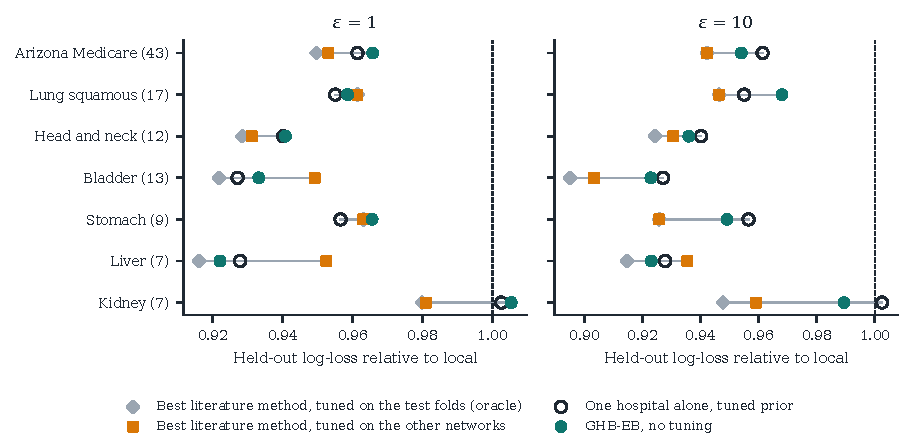
\includegraphics[width=\linewidth]{supplement/figures/real_final}
\caption{Seven real networks (hospitals in parentheses): held-out log-loss relative to local estimation, at $\epsilon=1$ and $\epsilon=10$. Teal: GHB-EB, which has nothing to tune. Orange: the best of twelve federated and personalized methods for that network, each tuned on the other seven networks. Grey: the same, tuned on the network's own held-out folds (oracle). Open circle: one hospital alone with a tuned prior. Choosing the best of twelve methods separately for every network is itself an advantage no hospital has.}
\label{fig:real-final}
\end{figure}

\begin{table}[t]
\caption{Seven real networks: held-out log-loss relative to local estimation, mean over the networks, for every method in the oracle arm (tuned on the network's own held-out folds) and the leave-one-network-out arm (tuned on the other networks); Wins: in how many of the seven networks GHB-EB, untuned, has a lower error than that method in the leave-one-network-out arm. $\ddagger$: no other hospital. Every method spends the same budget. Per-network values are in the supplement.}
\label{tab:real-final}
\scriptsize
\setlength{\tabcolsep}{4pt}
\begin{tabular}{@{}lrrrrrr@{}}
\toprule
 & \multicolumn{3}{c}{$\epsilon=1$} & \multicolumn{3}{c}{$\epsilon=10$}\\
\cmidrule(lr){2-4}\cmidrule(l){5-7}
Method & Oracle & Other networks & Wins & Oracle & Other networks & Wins\\
\midrule
\csname @@input\endcsname ../Collectively_Big_Locally_Small/supplement/results/tables/t_real_final.tex 
\bottomrule
\end{tabular}
\end{table}

\paragraph{With strong privacy, collaboration adds little for anyone} At $\epsilon=1$ (Figure~\ref{fig:real-final}, Table~\ref{tab:real-final}) GHB-EB, untuned, reduces the error of local estimation to \SimRFOneEB{} on average (\SimRFOneEBMin{} to \SimRFOneEBMax{} across networks). Tuned on the other networks, no literature method does better on average: the closest are Ditto (\SimRFOneDittoLono) and pFedMe (\SimRFOnePFedMeLono), and GHB-EB has a lower error than each of the twelve methods in at least four of the seven networks. Tuned on each network's own test folds, DP-FedAvg with fine-tuning and secure aggregation reaches \SimRFOneFTSAOrc, and the best of the twelve methods chosen afresh for every network beats GHB-EB in all but \SimRFOneBestOrcWins. But a single hospital that simply regularizes well does as well as any collaborative method: local estimation with a tuned prior reaches \SimRFOneLocLono, and GHB-EB is better than it in only \SimRFOneEBvsLocWins{} network. At this budget the privacy noise of each release is many times a hospital's own sampling error (Section~\ref{sec:heart-size} below), so the information these networks could share is mostly lost, whatever the method; what remains is regularization, which every method obtains in its own way.

\paragraph{With weaker privacy, the best tuned baselines lead by less than one percent} At $\epsilon=10$, collaboration starts to pay: GHB-EB (\SimRFTenEB) is better than local estimation with a tuned prior in \SimRFTenEBvsLocWins{} of the seven networks. Tuned on the other networks, pFedMe (\SimRFTenPFedMeLono) and DP-FedAvg with fine-tuning and secure aggregation (\SimRFTenFTSALono) are slightly more accurate on average than GHB-EB, Ditto ties it (\SimRFTenDittoLono), and the other nine methods are less accurate. Tuned on the test folds, DP-FedAvg with fine-tuning and secure aggregation leads by about two percent (\SimRFTenFTSAOrc).

\paragraph{Tuning is most of the baselines' advantage} The comparison turns on how the literature methods are tuned, and GHB has nothing to tune. Every baseline loses accuracy when its settings must come from other networks, and several become unstable: tuned on UCI Heart Disease alone, the mean error at $\epsilon=1$ becomes \SimRFOneFTSAUci{} for DP-FedAvg with fine-tuning and secure aggregation, \SimRFOneDittoUci{} for Ditto and \SimRFOnePFedMeUci{} for pFedMe, against \SimRFOneEB{} for GHB-EB, and FedRep diverges. A small hospital cannot tune on its own test patients, and has few patients to hold out for validation; the leave-one-network-out arm is the most a consortium could do for it, and there GHB-EB is the most accurate collaborative method at $\epsilon=1$ and within one percent of the best at $\epsilon=10$.

\paragraph{Two improvements, pre-registered} The first real-data run showed GHB, as reported, at the local level (\SimRFOneGHB{} at $\epsilon=1$): its fixed default prior $\mathcal{N}(0,2.5^2)$ is too loose for hospitals of a few dozen patients. \emph{GHB-EB} integrates the scale of the default prior out over $\{0.5,1,2.5\}$, weighting each scale by the hospital's own evidence exactly as $\tau$ is integrated out (Remark~\ref{rem:tau}); it needs no held-out data. It was developed on simulations with separate seeds and on UCI Heart Disease, and pre-registered with two criteria: improve on GHB in at least five of the seven networks, and raise no network's worst-hospital ratio by more than 0.1. It improved on GHB in \SimRFOneEBvsGHBWins{} networks but raised the worst ratio in the liver network from \SimRFOneLiverWorstGHB{} to \SimRFOneLiverWorstEB, through a hospital whose 22 patients all died; by its own rule it is reported as an extension, not as the default. Its gain at $\epsilon=1$ equals that of a local model with the same evidence-weighted prior, so it comes from regularization, not from borrowing. \emph{GHB-SA} replaces the per-hospital releases by two rounds of secure aggregation, so that the noise is added once to network sums whose sensitivity is set by one patient rather than by the smallest hospital. In development it removed about half of the privacy cost (supplement); on the real networks it improved on GHB-EB in only \SimRFOneSAvsEBWins{} of seven at $\epsilon=1$, with a worst ratio of \SimRFOneLiverWorstSA{} in the liver network, and failed its pre-registered criterion. With seven to seventeen hospitals, the heterogeneity statistic that GHB-SA privatizes as a single sum is too noisy, and its nominal public feature distribution biases it; at $\epsilon=10$ it matches GHB-EB (\SimRFTenSA{} against \SimRFTenEB). Both negative outcomes stand in the paper because they bound what GHB can do on networks of this size.

\paragraph{How much the size of a hospital matters}\label{sec:heart-size} The UCI Heart Disease data \cite{detrano1989international} are the classic multi-site benchmark of federated learning in healthcare \cite{ogierduterrail2022flamby}. They hold the records of patients referred for coronary angiography at four hospitals: the Cleveland Clinic (303 patients), the Hungarian Institute of Cardiology in Budapest (294), the University Hospitals of Zurich and Basel (123) and the VA Medical Center in Long Beach (200). The prevalence of angiographic coronary disease ranges from 36\% in Budapest to 93\% in Zurich and Basel, so the heterogeneity is real and large. Each hospital fits the pretest-probability model of coronary disease, a logistic regression on age, sex and chest-pain type (asymptomatic, anginal, or non-anginal as reference), the predictors that every site records completely. Age is scaled by public constants, $(\text{age}-55)/25$ clipped to $[-1,1]$, so that $\|x\|\le\sqrt{5}$ without fitting anything to the data. No published model is assumed, so GHB runs without an anchor: it releases the score at the public point 0, linearizes under the default prior, and gossips on a ring of four hospitals. The public feature distribution needed for the inversion is a nominal chest-pain clinic population (age $\mathcal{N}(55,9^2)$, 75\% men, 50\% asymptomatic, 30\% anginal pain), not the data, so every hospital is under a real case-mix shift. Evaluation is by repeated stratified five-fold cross-validation within each hospital (\SimRealHeartSplits{} splits). Each hospital trains on its training folds, subsampled to at most 20, 40 or 80 patients to emulate siloed smallness, or on all of them, and is scored by log-loss on its own held-out fold. The baselines are the same as in Simulation 15, with their hyperparameters chosen on the held-out folds themselves, which favours them. A local-only control, gradient descent on the hospital's own data with a tuned number of steps, separates what they gain by collaborating from what they gain by regularizing.

The result is mixed, and it is consistent with the theory. At $\epsilon=1$, no private method gains from collaboration in this network. GHB stays within 1\% of local estimation at every training size (\SimRealHeartTwentyGHBRel{} with at most 20 patients, \SimRealHeartAllGHBRel{} with all of them), and its worst hospital stays within a factor \SimRealHeartGHBWorstMax{} of its local error, at $\epsilon=5$ too. The privacy noise explains why. On the parameter scale, a hospital of 40 patients releases noise with a standard deviation about 26 times its own sampling error at $\epsilon=1$, and about 10 times at 300 patients. With only three other hospitals to average over, $M$ in Equation~\eqref{eq:M} dwarfs $\tau^2$ and Equation~\eqref{eq:borrowed} leaves almost nothing to borrow. GHB's posterior over $\tau$ and the hospital's own evidence detect this and fall back to local estimation, without any tuning. The tuned DP-FedAvg with fine-tuning appears to gain (\SimRealHeartTwentyFTRel{} with 20 patients). The local-only control gains exactly as much (\SimRealHeartTwentyLGDRel), because the chosen configuration is a single private round followed by 30 local steps, so its gain is early stopping tuned on the test folds, not borrowing. The Ditto-style model, pulled toward the average of the private releases, fails badly with small hospitals (\SimRealHeartTwentyDittoRel). Without privacy, GHB borrows: \SimRealHeartTwentyGHBNoDPRel{} of the local error with at most 20 training patients, \SimRealHeartFortyGHBNoDPRel{} with 40 and \SimRealHeartEightyGHBNoDPRel{} with 80, fading to \SimRealHeartAllGHBNoDPRel{} with all of them, as Equation~\eqref{eq:borrowed} predicts when $n_k$ grows. The nominal public feature distribution costs nothing: replacing it by the pooled empirical features gives \SimRealHeartTwentyGHBEmpRel{} with 20 patients. A single pooled model, also without privacy, is worse than local estimation on average at every size (\SimRealHeartTwentyGlobalRel{} to \SimRealHeartAllGlobalRel) and makes the Swiss hospital, with its 93\% prevalence, \SimRealHeartGlobalWorstMin{} to \SimRealHeartGlobalWorstMax{} times worse off. GHB without privacy keeps every hospital within 2\% of its local error. The lesson for deployment is the one the theory states. In a network of four hospitals of tens to a few hundred patients, a guarantee of $\epsilon=1$ per release leaves nothing to share, and GHB's value there is that it does no harm. Collaboration under privacy needs more hospitals (Simulation 17), joint release by small hospitals (Section~\ref{sec:privacy}) or a larger budget, and these data, unlike the eICU and similar collections, cannot test the regime of tens of hospitals that the simulations describe.

\begin{figure}[t]
\centering
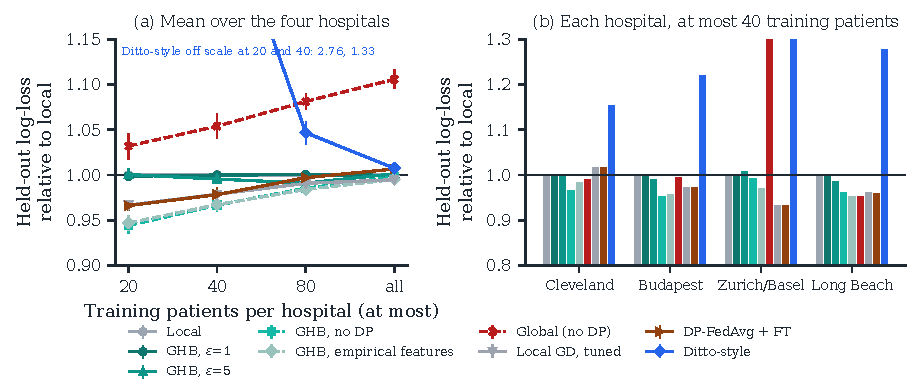
\includegraphics[width=\linewidth]{supplement/figures/real_heart}
\caption{UCI Heart Disease, four hospitals: held-out log-loss relative to local estimation (repeated stratified five-fold cross-validation, \SimRealHeartSplits{} splits; $\pm2$ paired standard errors). (a) Mean over hospitals against the number of training patients per hospital. (b) Each hospital, with at most 40 training patients (bars clipped at 1.3; values in Table~\ref{tab:real-heart} and the supplement). Dashed: without privacy. The baselines' hyperparameters are tuned on the held-out folds.}
\label{fig:real-heart}
\end{figure}

\begin{table}[t]
\caption{UCI Heart Disease: held-out log-loss relative to local estimation (two paired standard errors in grey) and the largest ratio of any hospital's held-out log-loss to its local one (Worst), by the number of training patients per hospital (\SimRealHeartSplits{} splits). First row: local log-loss (nats). DP-FedAvg + FT, Ditto-style and local GD are tuned on the held-out folds. $\dagger$: not private.}
\label{tab:real-heart}
\scriptsize
\setlength{\tabcolsep}{3.5pt}
\begin{tabular}{@{}lrrrrrrrr@{}}
\toprule
 & \multicolumn{2}{c}{$\le 20$ patients} & \multicolumn{2}{c}{$\le 40$} & \multicolumn{2}{c}{$\le 80$} & \multicolumn{2}{c}{All}\\
\cmidrule(lr){2-3}\cmidrule(lr){4-5}\cmidrule(lr){6-7}\cmidrule(l){8-9}
Method & Relative & Worst & Relative & Worst & Relative & Worst & Relative & Worst\\
\midrule
\csname @@input\endcsname ../Collectively_Big_Locally_Small/supplement/results/tables/t_real_heart.tex 
\bottomrule
\end{tabular}
\end{table}

\paragraph{What the real data say} Three findings hold across the eight networks. First, on networks of a few to a few dozen small hospitals with simple models, privacy at $\epsilon=1$ leaves little to share, and a hospital that regularizes well alone is as accurate as any collaborative method; the theory predicts this through Equations~\eqref{eq:M} and~\eqref{eq:borrowed}, and a network can check it from public quantities before it starts. Second, when collaboration does pay, GHB is competitive with the best federated and personalized methods without any tuning, and is the most accurate of them when their tuning must be transferred from other networks; tuned on the test data, which no hospital can do, the best of them lead by one to two percent. Third, the safety property holds where it matters: GHB never makes a hospital much worse off except at a hospital whose data are degenerate, where every method fails, and a single pooled model is the least safe of all methods. The real data do not show GHB dominating the literature, and the paper does not claim it.


%% ===================================================================
\section{Discussion}\label{sec:discussion}

\subsection{When to use GHB, and when not}\label{sec:when}

The evidence supports a plain reading of the theory. Collaboration pays when hospitals are small for their task and differ moderately; then Equation~\eqref{eq:borrowed} adds tens of virtual patients to every hospital. When they differ strongly, no method gains much, and integrating $\tau$ out keeps GHB near local estimation rather than below it. When they barely differ and a trusted pooling environment exists, a pooled model is better, and GHB can run inside it without noise.

Which protocol to run depends on what the network can provide. GHB needs secure summation among hospitals that do not collude, and in exchange calibrates its noise to the whole network and uses the hospitals' real case mix; it had the lowest mean error on the held-out cancer networks, by margins five networks cannot establish statistically. Its lead comes from fitting several related networks together, for instance one per disease, and survives networks of four hospitals and heads of 40 coefficients (Section~\ref{sec:real-stress}). A single network fitted alone, as in FLamby, gives it only the accuracy of a well-regularized hospital at strong privacy, and a consortium able to tune Ditto \cite{li2021ditto} or DP-FedAvg \cite{mcmahan2018learning} with fine-tuning and secure aggregation on comparable networks may do better under weak privacy. GHB-lite needs only honest-but-curious neighbours; it is the better choice when a public feature distribution matches the hospitals' patients and the network is large enough for per-hospital releases to be informative, as in the simulations and, partly, on FLamby. Where hospitals are known to share their base rates, borrowing the intercept, as GHB-lite does, is better. Before committing, a network can check from public quantities (sizes, budget and a prior guess of $\tau^2$) whether privacy leaves anything to share, with Equations~\eqref{eq:M} and~\eqref{eq:borrowed}.

\subsection{Deploying GHB in a real network}\label{sec:deploy}

Running GHB asks little of a hospital. Each one computes two sums over its own patients, the scores and the information of its head (\SimDeployNums{} numbers for the eight-coefficient cancer head, \SimDeployBytes{} bytes), adds its share of the noise and pairwise masks agreed with its neighbours, and exchanges masked values with them for some tens of gossip rounds; on the ring with two-hop links of Section~\ref{sec:experiments} that is about \SimDeployKB{} kB sent per hospital in total. Everything after the two releases is local: computing the leave-one-out prior and the evidence-weighted fit takes about \SimDeployMs{} ms per hospital on one processor core for the cancer networks. There is no server to procure or trust, and no training rounds to schedule: one release per model fit, repeated only when the model is refitted, with the costs of Section~\ref{sec:privacy} adding up under zero-concentrated accounting.

Three practical points remain. Secure summation must tolerate hospitals that drop out mid-protocol, which practical protocols do by secret-sharing each hospital's masks so that the survivors can remove them \cite{bonawitz2017practical}; a hospital that never answers simply contributes nothing, and the network's size $N$ is then the survivors' total. The channels can be those that networks already use for distributed analysis, such as the OHDSI network on the OMOP common data model \cite{hripcsak2015observational}, DataSHIELD \cite{gaye2014datashield} or the Personal Health Train \cite{beyan2020distributed,deist2020distributed}: they move analyses to the data, and GHB specifies what to compute and release through them. Finally, a network must agree on the head, the feature bound $G$, the budget $\epsilon$ and the collaboration graph before any release, and each hospital must document the processing, for instance in the data-protection impact assessment that the GDPR requires for health data \cite{gdpr2016}; under the European Health Data Space, a secure processing environment can host the summation instead of gossip \cite{ehds2025}.

\subsection{Limits}\label{sec:limits}

GHB protects against honest-but-curious hospitals and observers under Proposition~\ref{prop:ghbprivacy}; colluders weaken it, and GHB-lite is the option where collusion cannot be ruled out. A hospital that lies is not excluded: under GHB-lite a large lie inflates $\hat{\tau}^2$ and switches borrowing off (Simulation 12), while GHB, which has no per-hospital release in which to see a lie, relies on each hospital's evidence to stop borrowing from a network that conflicts with it; stronger adversaries need robust aggregation \cite{blanchard2017machine}. Refits compose and must be accounted for \cite{bun2016concentrated,mironov2017renyi}. The Gaussian analysis is asymptotic, and GHB's network estimate is one Newton step from the origin, accurate for the clinical heads studied here but not for heads far from it. The evidence has limits too. The design was chosen on development networks, and the held-out evaluation uses five networks of one source, with one outcome and an eight-coefficient head; the margins under weak privacy are small, and FLamby shows that other networks can reverse them. The baselines were tuned as well as a consortium could, and their oracle arm shows what more tuning buys, but other methods or grids could do better. On images the privacy unit is a patch, not a patient. Nothing here speaks to heads with many more coefficients, other outcomes, much larger networks or adversaries we did not test.

\subsection{Open problems}\label{sec:open}

\begin{enumerate}[leftmargin=*,itemsep=2pt]
\item \textbf{Private heterogeneity from joint releases.} GHB integrates $\tau$ over a fixed prior; GHB-lite learns it from releases that real networks made too noisy. A private estimate of $\tau^2$ from network sums would combine both strengths and let a hospital predict its benefit before joining.
\item \textbf{Topology design.} Since mixing depends on the spectral gap, choosing a few long-range agreements that maximize it is a concrete optimization problem.
\item \textbf{Weaker trust.} Shuffling or dropout-tolerant, collusion-detecting summation would keep network-level noise with less trust.
\item \textbf{Incentives.} Large hospitals gain least and contribute most; private data valuation \cite{ghorbani2019data} could support fair credit under regulation such as the European Health Data Space \cite{ehds2025}.
\item \textbf{Shift-aware borrowing.} Separating the transportable part of $\tau^2$ from the site-specific part, with causal invariance \cite{arjovsky2019invariant,castro2020causality}.
\item \textbf{Group fairness.} Borrowing can import or dilute disparities; Simulation 18 finds both effects small for GHB-lite, but parity of decisions would need further private releases \cite{salazar2023fairfate}.
\item \textbf{Procurement and strata.} Posterior variances could drive joint labeling across a consortium, and Equation~\eqref{eq:borrowed} applies to small subgroups as well as small sites.
\end{enumerate}

%% ===================================================================
\section{Conclusion}\label{sec:conclusion}

Networks of small hospitals without a trusted centre are the default form of healthcare, and they are poorly served by methods that assume a server, fit one model or must be tuned on data small hospitals do not have. Graph Hierarchical Borrowing gives each hospital almost the same number of virtual patients, pays the privacy cost once, in two sums over the whole network, runs over whatever agreements exist, and tunes nothing. On held-out cancer networks fitted together it had a lower mean error than every federated and personalized method tuned as a consortium could, at strong and weak privacy, and was level with them tuned on the test data under weak privacy, though five networks are too few to establish that lead statistically; the lead comes from borrowing across related networks, and a single network fitted alone gives it no more than a well-regularized hospital; across sixteen real data sets its gain over a hospital alone is established; on smaller benchmarks and on images it is competitive, leading in some settings and by small margins. Collaboration between small hospitals pays under privacy, by percent rather than by multiples, when the noise is calibrated to the network rather than to each hospital. Whether this holds for other outcomes, larger heads and larger networks is the main open question.

\begin{acks}
This work is funded by national funds through FCT, Foundation for Science and Technology, I.P., within the scope of the research unit UID/00326, Centre for Informatics and Systems of the University of Coimbra, \url{https://doi.org/10.54499/UID/00326/2025}.
\end{acks}

\bibliographystyle{../Collectively_Big_Locally_Small/ACM-Reference-Format-recovered}
\bibliography{../Collectively_Big_Locally_Small/references}

\end{document}
